
\section{Preface}
This chapter has been submitted to the BioRxiv preprint server with the following citation: Robin FB, Michaux JB, McFadden W, Munro EM.  Excitable RhoA dynamics drive pulsed contractions in the early C. elegans embryo.  BioRxiv (2016) Published online September 21, 2016. http://dx.doi.org/10.1101/076356.


This work was done in collaboration with Fran\c{c}ois Robin and Jonathan Michaux in Edwin Munro's lab at the University of Chicago.  Fran\c{c}ois performed the single-molecule imaging experiments, particle tracking, and statistical analyses documented in Figures 2.2, 2.3, 2.10, and 2.11.  Jon performed the remainder of experiments.  

My contribution was the analysis of the mathematical model presented in Figure \ref{fig:229} and Section \ref{sec:25}.  In addition, I wrote the code for fitting the model parameters using pulse time-series data, via either a piece-wise fitting approach or fitting the full function.  For a more detailed analysis of the modeling and fitting work the reader may refer to the Appendix \ref{chap:morepulse}.

\section{Abstract}
Pulsed actomyosin contractility underlies diverse modes of tissue morphogenesis, but the mechanisms that generate pulsed contractions are still poorly understood.  Here, we combine quantitative imaging with genetic perturbations and mathematical modeling to identify a core mechanism for pulsed contractility in early \textit{C.elegans} embryos.  We show that pulsed accumulation of actomyosin is governed almost entirely by local control of assembly and disassembly downstream of RhoA.  Pulsed activation and inactivation of RhoA precedes, respectively, the accumulation and disappearance of actomyosin, and persists in the near complete absence of Myosin II.  Autocatalytic activation of RhoA underlies rapid pulse initiation, while delayed accumulation of the RhoA GTPase activating proteins (GAPs) RGA-3/4 provides negative feedback to terminate each pulse. Mathematical models, tightly constrained by our experiments, confirm that this combination of positive and negative feedback is sufficient to generate locally pulsatile RhoA dynamics and reproduce the observed waveform of RhoA activation and RGA-3/4 acumulation. We propose that excitable RhoA dynamics are a common driver for pulsed contractility that can be tuned or coupled to actomyosin dynamics in different ways to produce a diversity of morphogenetic outcomes.


\section{Introduction}
Pulsed contractility is a widespread mode of actomyosin contractility expressed by many non-muscle cells in which transient accumulations of F-actin and Myosin II accompany local contractions of the cell surface. Pulsed contractions were first identified in the polarizing \textit{C.elegans} zygote  \cite{Munro:2004jk}, and have now been documented in a wide variety of embryonic and extra-embryonic epithelia  \cite{ Blanchard:2010kt, Rauzi:2010fs, David:2010bt, Martin:2009du, Solon:2009hg} and mesenchymal cells  \cite{Kim:2011cc}. A similar phenomenon known as cell shape oscillations have been observed in many cultured cells  \cite{Sedzinski:2011ef, Salbreux:2007fc, Kapustina:2008ds}. Pulsed contractions produce transient shape changes that can be biased or rectified in different ways to produce distinct morphogenetic outcomes such as tissue invagination  \cite{Martin:2009du}, tissue elongation  \cite{Rauzi:2010fs, Levayer:2013el}, epithelial tissue closure  \cite{Solon:2009hg} and wound healing  \cite{Razzell:2014eb}. During embryonic development, pulsed contractions may represent an adaptation to accommodate rapid cell and tissue deformations while maintaining overall tissue integrity  \cite{Vasquez:2014hv}. In other contexts, such as in many cultured cells, shape oscillations may represent an aberrant behavior that manifests when cells lose normal adhesion to their substrates  \cite{Salbreux:2007fc, Paluch:2005da}, or when microtubules are depolymerized  \cite{Kapustina:2013gc, Kapustina:2008ds, Rankin:2010je, Werner:2007bx, Piekny:2008jf, Bornens:1989wc} or when contractile tension is very high during cytokinesis  \cite{Sedzinski:2011ef}.

Despite their widespread occurrence and increasing evidence for their functional relevance, the mechanisms that initiate and terminate pulsed contractions remain poorly understood. From a dynamical perspective, pulsed contractions represent a form of excitable behavior, exemplified by action potentials in neuronal cells  \cite{Izhikevich:2007aa} or pulses of intracellular calcium release observed in many cell types  \cite{Goldbeter:1996aa}.  Theoretical studies highlight two key ingredients for excitability: positive feedback to drive rapid upswing in activity, and delayed negative feedback to bring it back down again. A key challenge is to identify the specific modes of positive and negative feedback that drive pulsed contractions.

Multiple forms of positive feedback could contribute to initiating pulsed contractions. For example, local actomyosin-based  contraction could promote further accumulation of actomyosin through mechanosensitive motor-filament binding  \cite{ FernandezGonzalez:2009hp,Ren:2009ep, Effler:2006hc, Schiffhauer:2016iy}, by enhancing actin filament assembly and/or stability  \cite{Hayakawa:2011dq, DeLaCruz:2015dj}, or by transporting and concentrating actomyosin and/or its upstream activators  \cite{Munjal:2015bx, Dierkes:2014tm}. Alternatively, dynamic clustering of F-actin and/or Myosin II by scaffolding proteins such as Anillin could promote Myosin II recruitment and focal contraction  \cite{Maddox:2005gd}. Finally, autocatalytic activation of upstream regulators such as RhoA could drive local excitation, independent of, or in addition to, myosin-based tension or network contraction  \cite{Zhang:2015bx, Munjal:2015bx, Bement:2015jp}. Similarly, multiple forms of delayed negative feedback could contribute to terminating pulses, including progressive buildup of steric or elastic resistance to further contraction  \cite{Dierkes:2014tm}, or contraction-mediated disassembly, or delayed recruitment of disassembly factors or inhibitors of Myosin II or RhoA  \cite{Munjal:2015bx, Kasza:2011ft, Bement:2015jp}.   

Here we combine quantitative imaging with experimental manipulations and mathematical modeling to identify the dynamical basis for pulsed contractility in the early \textit{C.elegans} embryo. Using single-molecule imaging and particle tracking analysis, we provide definite evidence that the initiation of pulsed contractions does not involve or require local redistribution of actomyosin or its upstream activators.  Instead, pulsed contractions are driven by local pulses of RhoA activity, which feed forward to control local accumulation of downstream targets F-actin, Myosin II and Anillin. We present evidence that pulsed accumulation of RhoA is governed by locally excitable RhoA dynamics: local autocatalytic activation of RhoA drives the rapid upswing of RhoA activity during pulse initiation, while F-actin-dependent recruitment of the redundantly acting RhoA GTPase activating proteins (GAPs) RGA-3/4 provide delayed negative feedback to terminate the pulse.  A minimal model, sharply constrained by our experimental data, suggests that this combination of feedback is sufficient to generate locally excitable or oscillatory RhoA dynamics and to explain quantitatively the temporal dynamics of RhoA activation and RGA-3/4 accumulation during each pulse. We propose that excitable RhoA dynamics defines a core mechanism for pulsed contractility and suggest that this mechanism may be tuned or filtered through downstream effectors to control the size or spacing or lifetime of pulsed contractions.  

\section{Results}
Pulsed contractions were originally described in \textit{C.elegans} during interphase in the polarizing zygote P0 (Figure \ref{fig:221}A-C, individual pulses indicated by white arrowheads in Figure \ref{fig:221}B;  \cite{Munro:2004jk}). In these cells, pulsed contractions are associated with transient deep invaginations of the cell surface (magenta arrows in Figure \ref{fig:221}A,B); this makes it more difficult to quantify local changes in density of cortical factors during individual pulses, because these measurements could be confounded by movements of the cortex in/out of the plane of focus. Therefore, we focused on pulsed contractions that occur at the two-cell stage in the anterior blastomere known as AB (Figure \ref{fig:221}D-F, individual pulses indicated by white arrowheads in Figure \ref{fig:221}E).  As in P0, pulsed contractions in AB involve transient accumulations of F-actin and Myosin II; they are associated with transient local contractions of the actomyosin cortex (Figure \ref{fig:221}F), but they are not associated with pronounced invaginations of the cell surface. 

%Figure \ref{fig:221}
\begin{figure}[!htbp]
\centering
\includegraphics[width=0.65\textwidth]{pulse/Figure2-1}
\caption[Actomyosin pulses in 1 and 2-cell stage embryos.]{\label{fig:221} \textbf{Actomyosin pulses in 1 and 2-cell stage embryos.} (A) Schematic view of the zygote P0 during early interphase.  Open circles represent the two pronuclei. (B) Micrograph of P0 in early interphase expressing GFP::UTR and NMY-2::RFP. In (A) and (B), white arrowheads indicate individual pulses and magenta arrows indicate membrane invaginations (ruffles). (C) Time evolution of a single pulse in P0. The square region measures $\sim$6.4$\mu$m by 6.4$\mu$m.  The time delay between frames is 6s for the first 6 frames, and 8s thereafter. (D) Schematic of an embryo at the early 2-cell stage, showing the anterior blastomere AB and the posterior blastomere P1.  Open circles represent the interphase nuclei. (E) Micrograph of an early two-cell stage embryo expressing GFP::UTR and NMY-2::RFP. White arrowheads indicate individual pulses (F) Time evolution of a single pulse. The square region measures $\sim$ 6.4$\mu$m by 6.4$\mu$m.  The time delay between frames is 2s for the first 5 frames, and 4s thereafter.}
\end{figure}


\subsection{Single-molecule analysis of actomyosin dynamics during pulsed contractions}
As a key step towards distinguishing different mechanisms for pulsed contractions, we used single-molecule imaging and single-particle tracking analysis to quantify the relative contributions of local turnover and redistribution to changes in F-actin and Myosin II density during individual pulses. As described previously  \cite{Robin:2014jf}, we used RNAi against GFP to obtain embryos expressing single molecule levels of Actin::GFP or of the non-muscle myosin heavy chain fused to GFP (NMY-2::GFP) over the endogenous proteins (Figure \ref{fig:222}A). We combined near-total internal reflection fluorescence (TIRF) imaging with single-molecule detection and tracking to measure the appearance, motion and disappearance of single-molecule speckles (Figure \ref{fig:222}A-C,  \cite{Robin:2014jf}). We assumed, with others  \cite{Watanabe:2002jb, Vallotton:2004kz}, that single molecule appearance and disappearance events report directly on local rates of filament assembly and disassembly.  We have shown previously that rates of turnover measured by single-molecule tracking agree well with those measured from single-molecule data by fitting kinetic models to photobleaching curves  ( \cite{Robin:2014jf}, Materials and Methods).

We then devised new methods to measure simultaneously: (a) single molecule appearance rates, disappearance rates and densities, and (b) local rates of cortical deformation, on a moving and deforming patch of cortex during individual pulsed contractions (Figure \ref{fig:2210}; see Materials and Methods for details). Briefly, we identified a reference frame for each pulse near the onset of contraction; within that frame, we identified a polygonal region of interest containing the contracting patch (dashed blue polygon in Figure \ref{fig:222}A; hereafter ``the patch''); we propagated the patch forward and backwards in time by extrapolating the displacements of tracked particles on or near its boundary (Figure 2.2D, Figure \ref{fig:2210}).   We then measured local deformation of the patch as frame-to frame changes in patch area, or by estimating a local strain rate from frame-to-frame displacements of the individual particles, with similar results in both cases (Figure 2.2E; Figure \ref{fig:2211}A-C; Materials and Methods).  At the same time, we measured the number of molecules and single-molecule appearance and disappearance rates within the patch over time (Figure 2.2F-H). Finally, we aligned single-molecule measurements with respect to the onset or termination of individual contractions to produce a dynamical signature of actin assembly, disassembly and deformation over the lifetime of a pulse (Figure \ref{fig:223}A-D; Figure \ref{fig:2211}D-F). These measurements allowed us to distinguish, cleanly, changes in single-molecule densities due to local assembly and disassembly from those due to local contraction (or expansion) of the cortical patch.


%Figure \ref{fig:222}
\begin{figure}[!htbp]
\centering
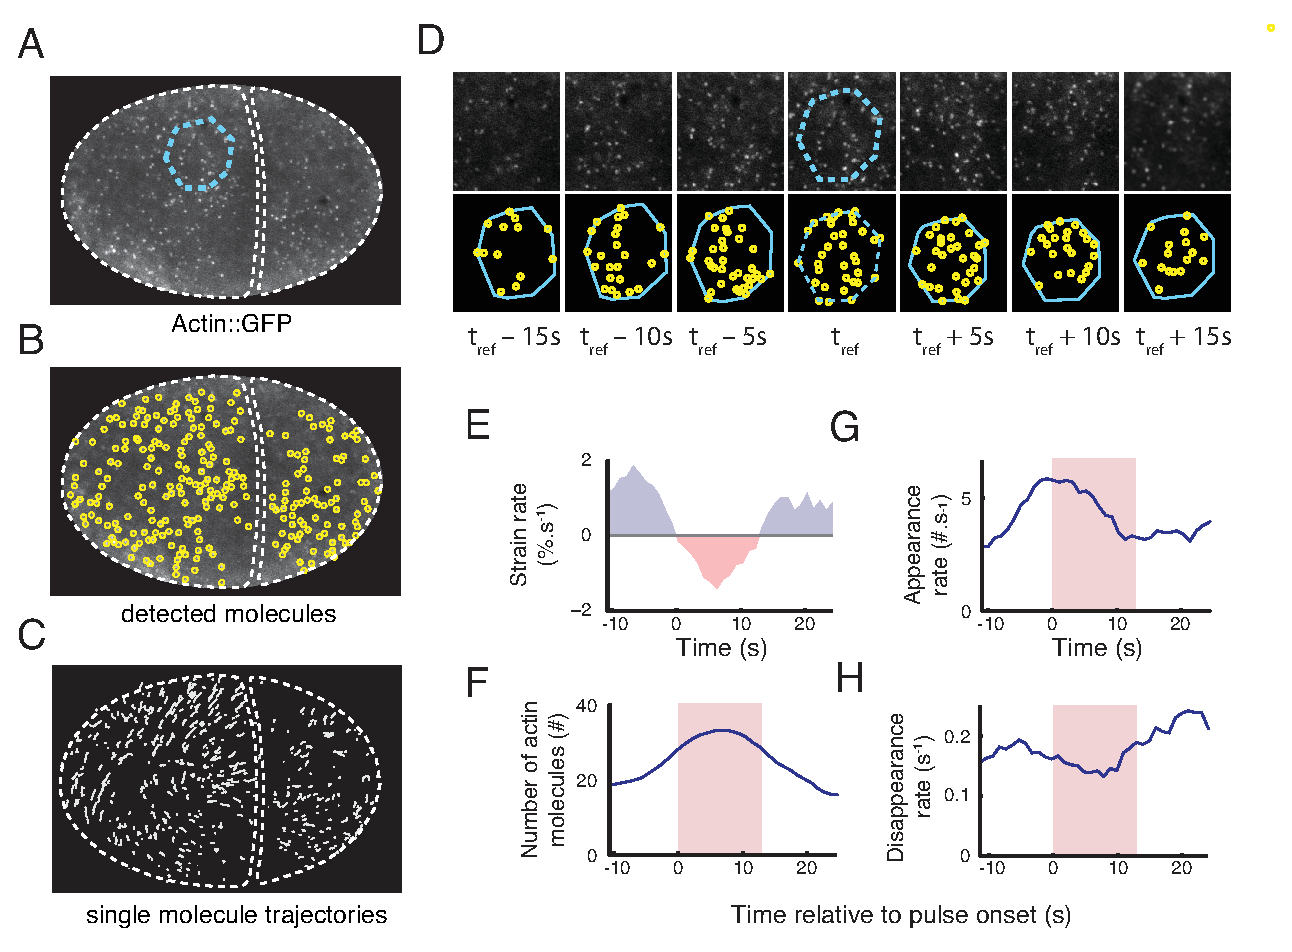
\includegraphics[width=1\textwidth]{pulse/Figure2-2}

\caption[Single-molecule analysis of actin network assembly, disassembly and deformation during individual pulsed contractions.]{\label{fig:222}\textbf{Single-molecule analysis of actin network assembly, disassembly and deformation during individual pulsed contractions.} One frame of a time lapse sequence taken from an embryo expressing low levels of Actin::GFP. A patch of cortex undergoing a pulse is identified from the time lapse sequence, and outlined in cyan. (B) Automatic particle detection of single-molecules from the image in (A). (C) Trajectories of the molecules displayed in (B) that were tracked for longer than 2s. (D) A polygonal region of interest identified at time $t = t_{ref}$, in (A) (dashed cyan polygon) is propagated forward and backward in time using the trajectories of tracked particles (see Materials and Methods). (E-H) Simultaneous measurements of single molecule dynamics and patch deformation over time. (E) Strain rate, measured using the particle-based method (see Materials and Methods). (F) Number of actin molecules in the patch. (G-H) Appearance rates (G) and disappearance rates (H) of actin molecules. Red shading in (F-H) indicates the time period in which the cortex is contracting locally (strain rate less than  0).}
\end{figure}


If pulses are initiated by positive feedback in which local contraction concentrates actomyosin and/or its upstream regulators, then the onset of actomyosin accumulation should coincide with the onset of contraction. Contradicting this expectation, we found that, on average, Actin:GFP began to accumulate $\sim$5s before the onset of contraction (Figure \ref{fig:223}B,F; Figure \ref{fig:2211}A-C), during a period of time in which the cortex was locally expanding (Figure \ref{fig:223}A). Approximately 30$\%$ of the total increase in Actin::GFP single molecule density measured during a pulse occurred before the onset of contraction (Figure \ref{fig:2211}A-C). This initial accumulation was due entirely to a net imbalance of assembly and disassembly (Figure \ref{fig:223}E): Before the onset of contraction, assembly rates increased (Figure \ref{fig:223}C) and disassembly rates decreased (Figure \ref{fig:223}D), leading to a sharp increase in the net rate of single molecule accumulation that peaked at the onset of contraction (Figure \ref{fig:223}E).  During the contraction phase itself, the rate of change in single-molecule densities was determined almost entirely by a net imbalance of assembly/disassembly, with a very minor (less than 6$\%$) contribution from contraction itself (Figure \ref{fig:223}E). Assembly rates decreased steadily, and disassembly rates increased steadily, such that a transition from net assembly to net disassembly  (and from increasing density to decreasing density) occurred $\sim$7s sec after the onset of contraction (Figure \ref{fig:223}E).  We obtained very similar results in embryos depleted of ARX-2, an essential subunit of the ARP2/3 complex (Figure \ref{fig:2212}), suggesting that our results are not biased by selective incorporation of Actin::GFP into branched vs unbranched F-actin  \cite{Chen:2012dx}.

Single-molecule analysis of GFP-tagged Myosin II (NMY-2::GFP) revealed local assembly/disassembly dynamics that were strikingly similar to those measured for GFP::Actin. (Figure \ref{fig:223}G-J). On average, the density of single molecules of NMY-2::GFP began to increase $\sim$6s before the onset of contraction during a period of local cortical expansion (Figure \ref{fig:223}H), and approximately 50$\%$ of this increase occurred before the onset of contraction. As observed for GFP::Actin, the upswing in Myosin II before the onset of a contraction was associated with both a sharp increase in appearance rates and a sharp decrease in disappearance rates (Figure \ref{fig:223}I,J); the net rate of increase peaked at the onset of contraction, and during the contraction phase, the appearance and disappearance rates returned steadily towards baseline levels.
In summary, we find that changes in actomyosin density during pulsed contractions are governed primarily by dynamic local imbalance of F-actin and Myosin II appearance and disappearance rates. A large fraction of the increase in F-actin and Myosin II density during each pulse occurs before the onset of contraction, and local contraction accounts for only a minor fraction of the subsequent density increase during the contraction phase itself. We conclude that changes in actomyosin density during pulsed contractions are governed primarily by dynamic modulation of assembly and disassembly, not by local clustering of these factors or by dynamical coupling of contraction and advection.


%Figure \ref{fig:223}
\begin{figure}[!htbp]
\centering
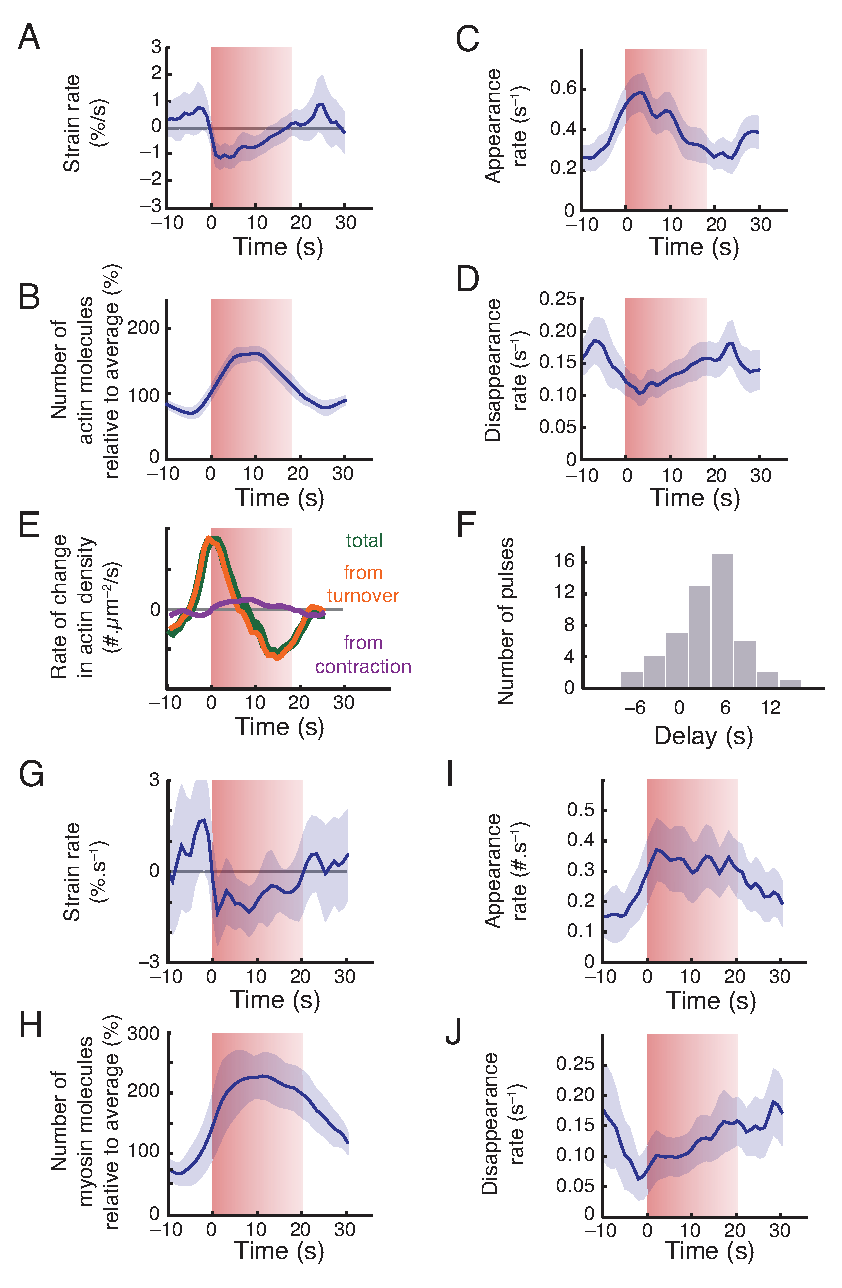
\includegraphics[width=0.5\textwidth]{pulse/Figure2-3}

\caption[Spatiotemporal modulation of assembly and disassembly drives transient accumulation of F-actin and Myosin II during pulsed contractions.]{\label{fig:223} \textbf{Spatiotemporal modulation of assembly and disassembly drives transient accumulation of F-actin and Myosin II during pulsed contractions.} (A-D) Data from individual pulses, aligned with respect to the onset of contraction and then averaged to display particle-based strain rate (A), numbers of actin molecules (scaled by the average number for each pulse) (B) appearance rate (C), and disappearance rate (D) versus time.  (E) Total rate of change in actin density (green) and the individual contributions to rate of change from turnover and surface contraction. (F) Distribution of time delays between the initiation of contraction and actin accumulation. Data in (A-F) were averaged over 42 pulses, collected in 8 embryos. (G-J) Average myosin dynamics synchronized with respect to time at which myosin density reached peak levels during a pulse, displaying particle-based strain rate (G), number of molecules (scaled to the average number for each pulse) (H), appearance rate (I) and disappearance rate (J) versus time. Data were averaged over 30 pulses, collected in 5 embryos. Error bars: 95$\%$ confidence interval. }
\end{figure}



\subsection{Pulsed activation of RhoA drives the pulsed accumulation of F-actin and Myosin II}
The observation that F-actin and Myosin II accumulate with very similar kinetics during pulsed contractions suggests that their accumulation is driven by a common upstream regulator. An obvious candidate is the small GTPase RhoA (encoded by \textit{rho-1} in \textit{C.elegans}), which recruits and/or activates downstream effectors including formins, Rho Kinase (ROCK) and Anillin to control F-actin assembly and Myosin II activation in a variety of cell types  \cite{Jaffe:2005kq, Piekny:2008jf}. RhoA activity is required for pulsed contractions in P0  \cite{Motegi:2006hi, Schonegg:2007if, Tse:2012fp}, and a biosensor for active RhoA derived from the RhoA Anillin (henceforth GFP::AHPH) localizes to contractile foci in the zygote  \cite{Tse:2011gd}. 

To determine if pulsed activation of RhoA accompanies pulsed contractions, we used a strain co-expressing GFP::AHPH  \cite{Tse:2012fp} with an RFP-tagged version of the myosin heavy chain (NMY-2::RFP) to co-monitor RhoA activity and Myosin II accumulation during individual pulses in AB.  We observed a striking correlation between pulsed accumulation of GFP::AHPH and NMY-2::RFP during individual pulsed contractions (Figure \ref{fig:224}A-C).  GFP::AHPH accumulated rapidly within a broad domain that prefigured the initial accumulation of NMY-2::RFP, reached a peak near the onset of visible contraction, and then began to disappear before NMY-2::RFP (Figure \ref{fig:224}B,C). The initial accumulation of GFP::AHPH was diffuse, whereas NMY-2::RFP accumulated as discrete particles that increased in number and size before contracting together into a smaller and tighter central domain. During the falling phase of each pulse, the diffuse pool of GFP::AHPH at the outer edges of the initial domain disappeared rapidly, while a smaller and more persistent fraction of GFP::AHPH co-localized with NMY-2::RFP particles in the central domain (yellow arrows in Figure \ref{fig:224}B; Figure \ref{fig:2213}).

%Figure 2.2.4
\begin{figure}[!htbp]
\centering
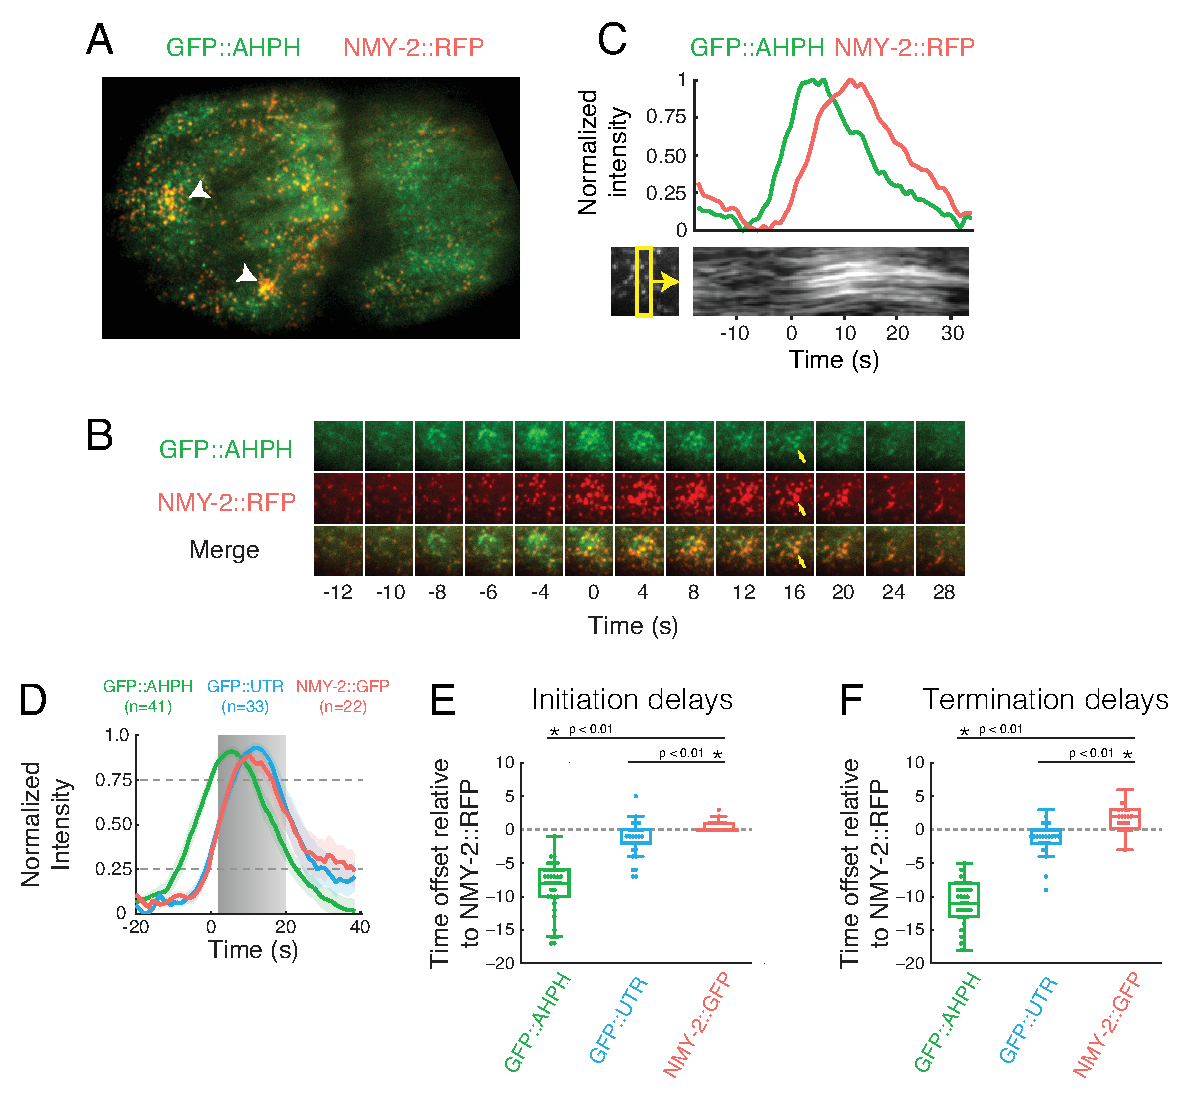
\includegraphics[width=0.6\textwidth]{pulse/Figure2-4}

\caption[Local pulses of RhoA activation underlie pulsed accumulation and disappearance of F-actin and Myosin II.]{\label{fig:224}\textbf{Local pulses of RhoA activation underlie pulsed accumulation and disappearance of F-actin and Myosin II.} (A) Micrograph of a 2-cell stage embryo expressing GFP::AHPH as a reporter for RhoA activity, and NMY-2::RFP. (B) Temporal dynamics of GFP::AHPH and NMY-2::RFP accumulation during a single pulse. The square region measures $\sim$5.3$\mu$m by 5.3$\mu$m. The time between frames is 2s for the first five frames, and 4s thereafter. (C) Above: Normalized fluorescence intensities of GFP::AHPH, and NMY-2::RFP. Below: A kymograph showing that local contraction (concerted movements of myosin puncta) begins after the accumulation of GFP::AHPH. The yellow box below left indicates the region used to generate the kymograph. (D) Comparison of averaged normalized fluorescence intensities vs time for active RhoA (GFP::AHPH), Myosin (NMY-2::GFP) and F-actin (GFP::UTR) from two-color data, co-aligned with respect to a common reference signal (NMY-2:RFP). Data were co-aligned with respect to the time at which NMY-2::RFP reaches 25$\%$ threshold. Hued regions report 95$\%$ confidence intervals. (E) Distribution of the delays between the onset of accumulation of NMY-2:RFP, and the onset of accumulation of GFP::AHPH, NMY-2::GFP and GFP::UTR. Onset of accumulation was measured as the time at which normalized probe intensity rose above 25$\%$ of its maximal level. (F) Distribution of the delays between the onset of disappearance of NMY-2:RFP, and the onset of disappearance of GFP::AHPH, NMY-2::GFP and GFP::UTR. Onset of disappearance was measured as the time at which normalized probe intensity fell below 75$\%$ of its maximal level. In boxplots, the central mark represents the median, the box indicates the 25th and 75th percentile, and the whiskers mark the minimum and maximum values}\end{figure}


To quantify these observations, we aligned data for multiple pulses from embryos co-expressing NMY-2::RFP and GFP::AHPH (see Materials and Methods). For each pulse, we smoothed and thresholded the NMY-2::RFP signal to identify a region of interest (ROI) containing high levels of NMY-2::RFP just before the onset of contraction (Figure \ref{fig:2212}A; Materials and Methods). We propagated this ROI forward and backwards in time (see Figure \ref{fig:2212}A, Materials and Methods), and then measured the mean intensities of the RFP and GFP signals within the ROI before, during and after the pulse (Figure \ref{fig:2212}B,C). We normalized these data with respect to the minimum (pre-contraction) and maximum intensities measured during this interval, then aligned data for multiple pulses with respect to the time point at which NMY-2::RFP reached 25$\%$ of its maximum intensity (Figure \ref{fig:224}D, Materials and Methods). These aligned data confirm that sharp increases and decreases in RhoA activity precede, respectively, the appearance and disappearance of NMY-2::RFP (Figure \ref{fig:224}D).  On average, GFP::AHPH reaches 25$\%$ of its maximum intensity 8.6 +/- 3.9 seconds before NMY-2::RFP (Figure \ref{fig:224}E), and falls below 75$\%$ of its maximum intensity 11.1 +/- 3.5 seconds before NMY-2::RFP (Figure \ref{fig:224}F).

We used the same approach to align data for embryos co-expressing NMY-2::RFP and either the F-actin binding domain of Utrophin fused to GFP (GFP::UTR); a marker for F-actin  \cite{Burkel:2007fj,Tse:2012fp}, or GFP::Anillin. Using NMY-2::RFP as the common reference to co-align data for NMY-2::RFP, GFP::AHPH, GFP::UTR and GFP::Anillin, we found that like Myosin II, F-actin and Anillin accumulate and dissipate during pulsed contractions with a significant delay relative to GFP::AHPH (Figure \ref{fig:224}D-F, Figure \ref{fig:2213}A-D). Thus local activation and inactivation of RhoA precedes and times the accumulation and disappearance of its downstream targets. 

Finally, we used the time points at which NMY-2::RFP intensities (Figure \ref{fig:224}D) and single molecule densities of Myosin::GFP (Figure \ref{fig:223}H) reached 25$\%$ of their peak values to align the time course of RhoA activation with respect to the onset of contraction as measured by single molecule imaging.  This analysis shows that RhoA activity peaks just before the onset of contraction (indicated by gray box in Figure \ref{fig:224}D) and thus local concentration of active RhoA by advection-contraction  \cite{Munjal:2015bx} cannot explain the rising phase of RhoA activation in \textit{C.elegans} embryos.  By extension, the same analysis reveals that RhoA activity peaks and begins to fall at a point where F-actin and Myosin II disappearance rates are at a minimum (Figure \ref{fig:223}D,J); thus factors other than cortical actomyosin disassembly drive the disappearance of active RhoA at the end of a pulse.

Using the same two-color image analysis, we confirmed that pulses of RhoA activity accompany pulsed contractions in the zygote P0. To remove the potentially confounding effects of large scale cortical flows that occur during zygotic polarization, we performed these measurements in embryos depleted of the centrosomal factor SPD-5  \cite{Munro:2004jk, Hamill:2002tw}, which exhibit pulsed contractions but lack cortical flows. In \textit{spd-5}(RNAi) P0 zygotes, as in wild-type AB cells, increases and decreases in local GFP::AHPH intensity preceded the rise and fall of NMY-2::RFP (Figure \ref{fig:2214}A-F) and to a lesser extent GFP::UTR (Figure \ref{fig:2214}D-F) and GFP::Anillin (Figure \ref{fig:2213}E-H).  As in AB, the initial accumulation of GFP::AHPH was broad and diffuse while a more persistent pool of GFP::AHPH remained concentrated within punctae that co-localized with NMY-2::RFP within a more central region of the initial domain (yellow arrows in Figure \ref{fig:2214}B). 

\subsection{Pulsed activation of RhoA does not require Myosin II.}
Recent studies suggested that active RhoA and Myosin II accumulate with similar timing during pulsed apical contractions in the \textit{Drosophila} germband, and that Myosin II activity is required for pulsed accumulation of active RhoA  \cite{Munjal:2015bx}. Our observation that active RhoA peaks before the onset of contraction rules out models in which local contraction concentrates RhoA, or its upstream activators, to initiate pulses. However, it remains possible that Myosin II activity is otherwise required for pulsed activation of RhoA. To test this possibility, we used RNAi to deplete the Myosin heavy chain NMY-2 in a strain co-expressing transgenic GFP::AHPH and NMY-2 tagged with mKate2 at the endogenous locus by CRISPR-mediated homologous recombination (NMY-2::mKate2, a kind gift of Dan Dickinson).  We used RNAi against NMY-2 to deplete NMY-2::mKate2 to the point where only a few single NMY-2::mKate particles could be detected at the P0 cortex using imaging conditions that allow robust detection of single molecules (Figure \ref{fig:225}A). Under these conditions, in \textit{nmy-2} RNAi zygotes, we still observed transient focal accumulations of GFP::AHPH (Figure \ref{fig:225}A,B).  These accumulations were roughly similar in size and spacing to those observed in \textit{spd-5} (RNAi) zygotes during polarity establishment, and many occurred on patches of cortex in which fewer than two discrete particles of NMY-2::mKate were detected, excluding any possible contribution from contractile tension generated by Myosin II (Figure \ref{fig:225}B). Aligning GFP::AHPH intensities vs time across many pulses in \textit{nmy-2}(RNAi) zygotes revealed a mean time course for AHPH accumulation and dissipation that is comparable to that measured for the diffuse pool of GFP::AHPH in \textit{spd-5} (RNAi) zygotes (Figure \ref{fig:225}C).  Indeed, pulses terminated more rapidly in \textit{nmy-2}(RNAi) than in \textit{spd-5} (RNAi) zygotes, implying that neither Myosin II activity nor its inhibition is required for rapid pulse termination. We conclude that Myosin II is not required for locally pulsatile activation of RhoA in \textit{C.elegans} embryos, although myosin activity may shape spatiotemporal pulse dynamics (see Discussion).

%Figure 2.2.5
\begin{figure}[!htbp]
\centering
\includegraphics[width=1\textwidth]{pulse/Figure2-5}

\caption[Myosin II is not required for the pulsed activation of RhoA.]{\label{fig:225}\textbf{Myosin II is not required for the pulsed activation of RhoA.} (A) Comparison of pulse dynamics in zygotes expressing GFP::AHPH and NMY-2::mKATE and treated with either \textit{spd-5}(RNAi) or \textit{nmy-2}(RNAi). Top panels show myosin localization (NMY-2::mKATE), middle panels show RhoA activity (GFP::AHPH). Bottom panels are kymographs showing GFP::AHPH dynamics over time.  Dashed yellow rectangles in middle panel indicate the regions from which the kymographs were made. Vertical yellow arrows indicate a region undergoing repeated pulses. Intensities were scaled identically for \textit{spd-5}(RNAi) and \textit{nmy-2}(RNAi) zygotes. (B) Top: Mean intensities of NMY-2::mKATE (red) and GFP::AHPH (green) vs time for a single pulse in an \textit{nmy-2}(RNAi) zygote. Bottom: sequential snapshots of the region undergoing the pulse showing NMY-2::mKATE (red) and GFP::AHPH (green) distributions. Yellow arrowheads indicate the  1-2 particles that can be detected in the region undergoing a pulse. (C) Mean intensity of GFP::AHPH over time in \textit{nmy-2}(RNAi) and \textit{spd-5}(RNAi) zygotes, aligned with respect to the time at which the normalized signal reaches 25$\%$ of its maximum value.  For \textit{spd-5} (RNAi) zygotes, the signal was measured either within the entire boxed region in which each pulse occurred  or at its periphery (see Figure \ref{fig:221}2 for details). Hued regions report 95$\%$ confidence intervals.}
\end{figure}



\subsection{RhoA feeds back locally to promote its own activity and this is required for pulse initiation.}
A recent study described propagating cortical waves of RhoA activity in echinoderm oocytes and frog embryos; these appear to be driven by locally excitable RhoA dynamics in which RhoA feeds back positively to promote its own activation and negatively, through local F-actin assembly, to promote delayed inactivation  \cite{Bement:2015jp}.  We hypothesized that a similar combination of positive and negative feedbacks could drive local pulses of RhoA activity in \textit{C.elegans} embryos.  Plotting the rate of change in GFP::AHPH intensity vs intensity during the rising phase of individual pulses in either P0 or AB cells revealed a sharp increase in the rate of RhoA activation with increasing RhoA (Figure \ref{fig:226}A). This is consistent with a scenario in which active RhoA feeds back positively to promote further activation of RhoA.  However, it could also reflect pulsed activation of RhoA (without feedback) by an upstream activator.  To distinguish these possibilities, we used RNAi to progressively deplete embryos of RhoA. If the time course of RhoA activation is dictated by an upstream activator, we should observe pulsed accumulation of GFP::AHPH as long as it remains detectable at the cortex. In contrast, if positive feedback of RhoA onto itself drives pulse initiation, then there should be an abrupt loss of pulsing below a threshold level of RhoA.  Consistent with the latter expectation, we observed an abrupt transition from pulsed to non-pulsed RhoA accumulation after $\sim$ 12 hours of feeding (Figure \ref{fig:226}B,C).  In zygotes that lacked pulsed RhoA accumulation, we could still readily detect robust RhoA-dependent cortical flows  \cite{Motegi:2006hi, Schonegg:2006ed} during polarity establishment (dashed yellow lines in Figure \ref{fig:226}B) and localized accumulation of active RhoA prior to cytokinesis (cyan arrowheads in Figure \ref{fig:226}B).  Together, these observations support the idea that RhoA feeds back positively to amplify its own activation and that sufficiently strong feedback is required to generate local pulses of high RhoA activity. 


%Figure 2.2.6
\begin{figure}[!htbp]
\centering
\includegraphics[width=1\textwidth]{pulse/Figure2-6}

\caption[RhoA activation is autocatalytic.]{\label{fig:226}\textbf{RhoA activation is autocatalytic.} (A) The time derivative of normalized RhoA activity (GFP::AHPH) plotted vs normalized activity during the early phase of pulse initiation in P0 (top panel, n = 40 pulses) and AB (bottom panel, n = 41 pulses). Error bars: 95$\%$ confidence interval. (B-C) Analysis of pulse dynamics in embryos progressively depleted of RHO-1 by RNAi.  (B) Top panels show GFP::AHPH distributions in interphase embryos from mothers subjected to no (wild type), 10 hours and 13 hours of \textit{rho-1}(RNAi). Middle panels  show kymographs from the same embryos illustrating spatiotemporal dynamics of GFP::AHPH  from interphase through cytokinesis.  Dashed yellow lines indicate approximate pattern of cortical flow.  Cyan arrowheads indicate accumulation of GFP::AHPH just prior to cytokinesis.  (C) Timeline indicating the presence (magenta circles) or absence (cyan circles) of pulsing in embryos treated with \textit{rho-1}(RNAi) for the indicated times, revealing an abrupt transition from pulsing to no pulsing at $\sim$12 hours post-treatment.}
\end{figure}

\subsection{Delayed accumulation of the Rho GAPs RGA-3/4 underlies pulse termination.}
What terminates RhoA activity during each pulse? Our results imply that local termination of RhoA activity at the end of a pulses does not require Myosin II activity or (by extension) its local inhibition by Myosin phosphatase  \cite{Piekny:2002vx, Piekny:2003iv}, nor is it timed by cortical disassembly. Previous studies identified the redundant RhoA GAPs RGA-3 and RGA-4 as inhibitors of RhoA activity during polarization and cytokinesis  \cite{Schonegg:2007if, Zanin:2013el, Schmutz:2007jq, Tse:2012fp}. A YFP-tagged RGA-3 transgene accumulates at the cortex in early embryos  \cite{Schonegg:2007if}, and simultaneous depletion of RGA-3 and RGA-4 leads to hyper activation of RhoA and hypercontractility during zygotic polarization  \cite{Schonegg:2007if, Schmutz:2007jq, Tse:2012fp}.  We wondered, therefore, if RGA-3/4 could provide negative feedback to terminate RhoA activity during individual pulses.
To test this possibility, we first imaged embryos co-expressing GFP::RGA-3 and NMY-2::mKATE. Focusing on AB, and using 2-color analysis as above, we confirmed that GFP::RGA-3 is present throughout the cortex, but accumulates locally during individual pulsed contractions (Figure \ref{fig:227}A-C). Significantly, GFP::RGA-3 and NMY-2::mKATE accumulated with very similar timing (Figure \ref{fig:227}B). Using NMY-2::mKATE and NMY-2::RFP  as common signals to co-align data for GFP::AHPH and GFP::RGA-3, we inferred that, on average, GFP::RGA-3 accumulates with a $\sim$6 sec delay relative to GFP::AHPH. The rate of RhoA activation peaks before the onset of GFP:RGA-3 accumulation, and rapid accumulation of GFP::RGA-3 coincides with deceleration and then reversal of RhoA activation (Figure \ref{fig:227}C, bottom). Together, these observations suggest that delayed accumulation of RGA-3/4 plays a key role in terminating each pulse of RhoA activity. To test this further, we created a strain in which GFP::AHPH and NMY-2::mKATE were co-expressed in \textit{rga-3;rga-4} (hereafter \textit{rga-3/4}) double mutant embryos  \cite{Zanin:2013el}. Consistent with previous reports  \cite{Schonegg:2007if, Zanin:2013el, Schmutz:2007jq, Tse:2012fp}, during polarity establishment in P0 in \textit{rga-3/4} double mutant embryos, we observed hyper-accumulation of GFP::AHPH and hypercontractility that was characterized by a sequence of convulsive contractions of the anterior cortex and rapid anterior directed cortical flows (Figure \ref{fig:227}D, 2nd column).  However, we could no longer detect local pulses of GFP::AHPH in these embryos.  In principle, this could be because rapid flows sequester factors required for pulsed contractility to the extreme anterior pole. To exclude this possibility, we used partial depletion of the myosin regulatory light chain (MLC-4) to attenuate contractility and cortical flows in \textit{rga-3/4} double mutant zygotes or in control zygotes that were doubly heterozygous for \textit{rga-3} and \textit{rga-4} (Figure \ref{fig:227}D).  In control zygotes partially depleted of MLC-4, cortical flows were sharply reduced, but pulsed accumulation of GFP::AHPH could be readily detected (Figure \ref{fig:227}D, 3rd column). By contrast, in \textit{rga-3/4} double mutant zygotes partially depleted of MLC-4, cortical flows during polarity establishment phase were slower than observed in wild type embryos; GFP::AHPH was uniformly enriched, but we did not observe local pulses of GFP::AHPH accumulation (Figure \ref{fig:227}D, 4th column).  Together, these data suggest that negative feedback through delayed accumulation of RGA-3/4 plays a key role in terminating local pulses of RhoA activity.


%Figure 2.2.7
\begin{figure}[!htbp]
\centering
\includegraphics[width=0.75\textwidth]{pulse/Figure2-7}

\caption[Delayed accumulation of RGA-3/4 mediates negative feedback required for pulse termination.]{\label{fig:227}\textbf{Delayed accumulation of RGA-3/4 mediates negative feedback required for pulse termination.} (A) Micrograph of a 2-cell stage embryo expressing GFP::RGA-3 (green) and NMY-2::RFP (red). (B) Temporal dynamics of a single pulse. The square region measures 6.4$\mu$m by 6.4$\mu$m. (C) Top: Averaged normalized fluorescence intensities vs time for NMY-2::RFP and GFP::RGA-3 from two-color data, co-aligned with respect to the time at which NMY-2::RFP reaches 25$\%$ threshold. The averaged normalized fluorescence intensity of GFP::AHPH, co-aligned with NMY-2::RFP.  Bottom: The averaged time derivative of the normalized GFP::AHPH intensity, again co-aligned using NMY-2::RFP.  Hued regions report 95$\%$ confidence intervals. (D) (top panels) Distributions of GFP::AHPH during interphase in zygotes  with the indicated genotypes.  (bottom panels) Kymographs showing patterns of GFP::AHPH distribution and redistribution during interphase for the same genotypes. Micrographs of 1-cell stage embryos expressing GFP::AHPH. RhoA exhibits pulsatile activity in \textit{rga-3/4}(+/-) embryos (control n=4 embryos, \textit{mlc-4} RNAi n=6 embryos) but not \textit{rga-3/4}(-/-) embryos (control n=9 embryos, \textit{mlc-4} RNAi n=8 embryos).}
\end{figure}

Recent work suggests that F-actin accumulation mediates delayed inhibition of RhoA activity in echinoderm and frog oocytes and embryos  \cite{Bement:2015jp}.  We wondered if F-actin might play a similar role in \textit{C.elegans} embryos by mediating recruitment of RGA-3/4.  Consistent with this possibility, two-color imaging of GFP::RGA-3 and mCherry::Lifeact  (a marker for F-actin   \cite{Pohl:2012bg}) revealed extensive co-localization of RGA-3 and F-actin in both P0 and AB (Figure \ref{fig:228}A).  A substantial fraction of GFP::RGA-3 co-localized with mCherry::Lifeact in extended linear structures that presumably represent actin filaments and/or small filament bundles. Treating permeabilized zygotes  \cite{Carvalho:2011ce, Olson:2012cs} with Latrunculin A to depolymerize F-actin lead to a profound loss of cortical GFP::RGA-3, supporting the idea that F-actin plays a key role in recruiting RGA-3/4 to the cortex during individual pulses (Figure \ref{fig:228}B).




%Figure 2.2.8
\begin{figure}[!htbp]
\centering
\includegraphics[width=1\textwidth]{pulse/Figure2-8}

\caption[Cortical RGA-3/4 localization depends on F-actin]{\label{fig:228}\textbf{Cortical RGA-3/4 localization depends on F-actin} (A) Micrographs of P0 (top) and AB (bottom) embryos co-expressing GFP::RGA-3 and mCherry::LifeAct. (B) Zygote co-expressing GFP::RGA-3 and mCherry::LifeAct before (top) and $\sim$90s after (bottom) treatment with 10µM Latrunculin A.}
\end{figure}



\subsection{Fast positive and delayed negative feedback involving RhoA and RGA-3/4 can account quantitatively for locally pulsatile RhoA dynamics.}
\label{sec:25}
Our data suggest that locally excitable RhoA dynamics could arise independently of myosin activity through a combination of fast positive feedback on RhoA activity and delayed negative feedback via local recruitment of RGA-3/4 (Figure \ref{fig:229}A).  To ask if this combination of feedback loops is sufficient to generate locally pulsatile activity, we formulated a simple ordinary differential equation model, describing local rates of change in RhoA and RGA-3/4, based on the following assumptions:  (a)  RhoA is activated at a basal rate, and feeds back positively to promote further RhoA activation, (b) RhoA feeds forward through F-actin assembly to promote local, reversible, association of RGA-3/4 with the cortex and (c) RGA-3/4 acts as a GAP to promote local inactivation of RhoA. Consistent with our experimental observations (Figure \ref{fig:226}A), we assumed that autoactivation of RhoA is a saturating function of RhoA activity, represented by a Hill function with Hill coefficient n = 1. We assumed that inactivation of RhoA by RGA-3/4 obeys Michaelis-Menten kinetics. To account for the observed delay between an increase in RhoA and the sharp onset of RGA-3/4 accumulation (Figure \ref{fig:227}C), we assumed ultrasensitive dependence of RGA-3/4 accumulation rate on RhoA, with the steepness of the response governed by an exponent m (see Materials and Methods for mathematical details). 



%Figure 2.2.9
\begin{figure}[!htbp]
\centering
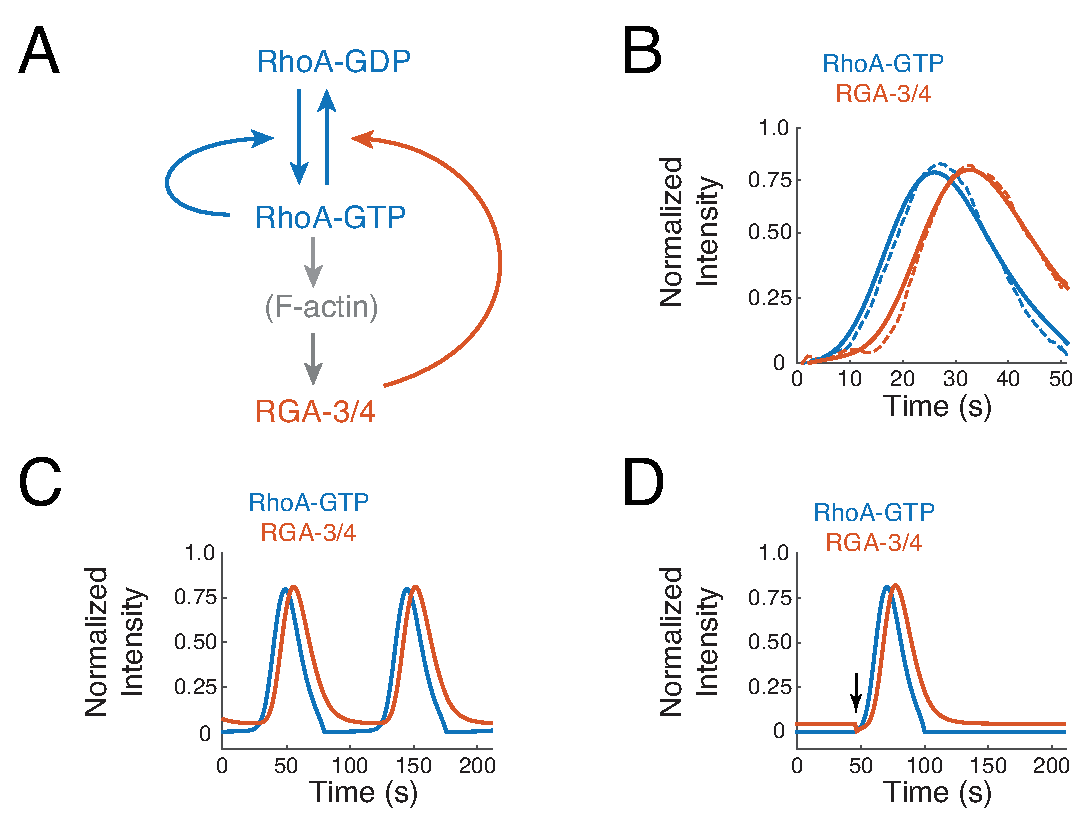
\includegraphics[width=1\textwidth]{pulse/Figure2-9}

\caption[Autocatalytic RhoA activation and delayed negative feedback through RGA-3/4 is sufficient to produce locally excitable RhoA dynamics.]{\label{fig:229}\textbf{Autocatalytic RhoA activation and delayed negative feedback through RGA-3/4 is sufficient to produce locally excitable RhoA dynamics.} (A) Schematic representation of the simple mathematical model used to model RhoA pulse dynamics. (B) Comparison between measured (dashed lines) and simulated (solid lines) pulse dynamics for the case in which n = 1, $k_{r}^0 = 0.005$, $k_{p}^0 = 0.006$.  The remaining model parameters were estimated by fitting data ($m=1.5289$, $K_{fb}=0.4581$, $K_{GAP}=0.001$, $k_{r}^{ass}=0.1592$, $k_{r}^{diss}=0.1101$; see Materials and Methods for details).  (C) Simulation dynamics for the parameter values in (B) are oscillatory, with pulses occurring at regular intervals.  (D)  A small change in the basal RhoA activation rate from $k_{p}^0 = 0.006$ to $k_{p}^0 = 0.004$ results in excitable dynamics in which a stable rest state can be destabilized by a transient reduction of RGA-3/4 (vertical black arrow) to trigger a single pulse of RhoA activity.}
\end{figure}



We set values for basal RhoA activation and RGA-3/4 recruitment rates based on the slow rates of increase in GFP::AHPH and GFP::RGA-3 observed before the sharp upswing of each pulse (Figure \ref{fig:227}C). Then we estimated values for the model’s remaining parameters by fitting the relationships between the local rates of RhoA activation and RGA-3/4 recruitment and the local densities of RhoA and RGA-3/4 inferred from averaged and co-aligned GFP::AHPH and GFP::RGA-3 intensities  (Figure \ref{fig:227}C; see Materials and Methods for details).   For these choices of parameters,  without any further adjustments, the model predicts oscillatory dynamics, with a pulse waveform that matches closely that measured for pulses in AB cells (Figure \ref{fig:229}B,C).  

Interestingly, the dynamics could be tuned by small decreases in the basal RhoA activation rate (Figure \ref{fig:229}D) or small increases in the basal RGA-3/4 recruitment rate (not shown), into a regime in which the dynamics are excitable - i.e., there is a stable state and a transient local input is required to trigger a pulse of RhoA activity (Figure \ref{fig:229}D).  This is consistent with our observations in \textit{nmy-2}(RNAi) embryos that some patches of cortex are quiescent while others exhibit repeated pulses of activity at regular intervals (yellow arrows in Figure \ref{fig:225}A). We conclude that a simple combination of positive and negative feedback loops, coupling local RhoA activity and RGA-3/4 accumulation, is in principle sufficient to explain pulsatile RhoA dynamics in early \textit{C.elegans} embryos, independent of actomyosin contractility.





\section{Discussion}
Pulsed contractility is a widespread mode of actomyosin contractility, but its mechanistic basis has remained poorly understood  \cite{Levayer:2012bu, Gorfinkiel:2016bv}. Current models for pulsed contractility invoke mechanochemical feedback in which contractile forces produced by Myosin II couple in different ways with actomyosin assembly/disassembly to drive excitable or oscillatory dynamics. Proposed feedback mechanisms include tension-dependent motor binding kinetics  \cite{Ren:2009ep, Effler:2006hc, Luo:2012bl}, tension-dependent filament assembly/stabilization  \cite{Hayakawa:2011dq, DeLaCruz:2015dj} or disassembly  \cite{Machado:2014fx}, tension-dependent activation of Myosin II via Ca++  \cite{Kapustina:2008ds} or RhoA  \cite{Koride:2014hp}, or modes of feedback in which local contraction advects and concentrates actomyosin and/or its upstream activators  \cite{Bois:2011kx, Kumar:2014ux, Munjal:2015bx}.  Here, we have identified a mechanism for pulse generation that does not require force production or redistribution of cortical factors by Myosin II.  Using single molecule imaging and particle tracking analysis, we have shown that the rapid initial accumulation of F-actin and Myosin II begins well before the onset of contraction, at a time when the cortex is locally expanding; Redistribution of actomyosin by local contraction makes a minor contribution to the overall accumulation of actomyosin during each pulse.  Instead, our data show that pulsed accumulation and disappearance of F-actin and Myosin II are determined primarily by local modulation of their assembly/recruitment and disassembly. Using two-color imaging, we have shown that during each pulse, active RhoA begins to accumulate well before its downstream targets F-actin, Myosin II and Anillin. Active RhoA nearly reaches its peak level before the onset of contraction (Figure \ref{fig:224}D), and then it begins to disappear well before its downstream targets. Significantly, locally pulsed activation of RhoA continues to occur on patches of cortex that contain only a few (1-2) particles of Myosin II, which presumably are insufficient to produce local contractile stress. Thus a Myosin-independent RhoA pulse-generator underlies pulsed contractility in early \textit{C.elegans} embryos.

The pulses of RhoA activity described here and in other contexts  \cite{Munjal:2015bx, Bement:2015jp, Mason:2016bs} are strikingly reminiscent of excitable behaviors found in other systems, such as action potentials in neuronal  \cite{Izhikevich:2007aa} or cardiac cells  \cite{Luo:1991vz}, or transient pulses of intracellular calcium release  \cite{Goldbeter:1996aa}, or pulses of actin assembly observed in motile cells  \cite{Weiner:2007cl}. Theoretical studies highlight two key ingredients for excitable dynamics: fast positive feedback and delayed negative feedback  \cite{Strogatz:1994tz}. The sharp acceleration of active RhoA accumulation that we observe during the early rising phase of individual pulses is a dynamical signature of fast positive feedback in which RhoA promotes its own activity. Stronger evidence that RhoA participates in a positive feedback loop that is essential for pulsing comes from our observation that depletion of RhoA below a certain threshold leads to an abrupt loss of pulsed contractions, while having minimal effects on other RhoA-dependent functions such as cortical flow during polarization \cite{Motegi:2006hi, Schonegg:2006ed} or cytokinesis  \cite{Loria:2012ks}. 

The mechanism for this feedback remains unclear.  Because the initial acceleration of RhoA activation occurs before any visible accumulation of Myosin II, Anillin or F-actin, it is unlikely that accumulation of these downstream targets makes a significant contribution to positive feedback.  A more likely possibility is that RhoA feeds back through one or more of its upstream activators, such as ECT-2, CYK-4 and NOP-1  \cite{Tse:2012fp}.  For example, during cytokinesis, active RhoA can act as a cofactor to promote transactivation of the RhoGEF ECT-2 by the RhoGAP CYK-4  \cite{Zhang:2015bx}.  While CYK-4 is not required for pulsed activation of RhoA during polarization  \cite{Tse:2012fp}, it is possible that RhoA could feedback through NOP-1, a protein of unknown activity that is required for RhoA activation during interphase in P0 and AB  \cite{Tse:2012fp}. Identifying the molecular mechanism(s) for this feedback is an important goal for future studies.


Our data suggest that the redundantly acting RhoGAPs RGA-3/4 play a key role in providing the delayed negative feedback that terminates RhoA pulses. RGA-3/4 act as GAPs towards RHO-1 in vitro  \cite{Schonegg:2007if}, and loss of RGA-3/4 leads to hyperactivation of RhoA in vivo  \cite{Tse:2012fp}.  We find that during each pulse, RGA-3 accumulates with a delay of $\sim$6 seconds relative to active RhoA. Significantly, the rate of active RhoA accumulation peaks, and begins to fall, just as GFP::RGA-3 begins to accumulate, suggesting that rapid accumulation of RGA-3/4 plays a key role in timing the end of each RhoA pulse. Consistent with this possibility, pulsatile RhoA activation is completely abolished in \textit{rga-3/4} double mutant zygotes, even when contractility is attenuated to prevent sequestration of RhoA activators by hyperactive cortical flow.  A similar dependence of pulsatility on a RhoA GAP has recently been reported in the context of ventral furrow invagination in \textit{Drosophila}  \cite{Mason:2016bs}.

Together, these data suggest a model for locally excitable RhoA dynamics in which RhoA feeds back positively to promote its own activation, and feeds back negatively with a delay through RGA-3/4 to promote its own inactivation. Indeed, when we formulate this model mathematically, and constrain model parameter values to match the local dependencies of RhoA and RGA-3/4 accumulation rates on levels of RhoA and RGA-3/4 inferred from two-color imaging data, the model predicts locally pulsatile RhoA dynamics, and small tunings of the model’s parameters  mediate interconversion between excitable dynamics and spontaneous oscillations.  This simple modeling exercise establishes an internally consistent hypothesis for pulsatile contractility that can be confirmed and extended by future experiments.

What governs the recruitment of RGA-3/4 during each pulse?  We have found that GFP::RGA-3 co-localizes broadly and extensively with cortical F-actin in both P0 and AB. RGA-3/4 accumulates with the same timing as F-actin during each pulse, and depolymerizating F-actin abolishes this accumulation.  This suggests a specific mechanism for delayed recruitment of RGA-3/4 in which RhoA promotes increased local F-actin assembly (potentially through the formin CYK-1  \cite{Severson:2002ve}), and F-actin in turn recruits RGA-3/4.  Interestingly, a recent study \cite{Bement:2015jp} suggests that RhoA and cortical F-actin form an excitable circuit, with RhoA as activator and F-actin as inhibitor, that propagates cortical waves of RhoA activity and F-actin assembly in oocytes and embryonic cells of frogs and echinoderms.  The mechanism(s) by which F-actin feeds back to inactivate RhoA in these cells remains unknown, but our observations in \textit{C.elegans} support to the idea, proposed by Bement et al, 2015, that a  RhoGAP homologous (or analogous) to RGA-3/4 may be recruited by F-actin to mediate negative feedback in frog and echinoderm cells. A similar circuit design may underlie the propagation of actin waves observed in many motile cells (reviewed in  \cite{Allard:2013if}).

It is also interesting to compare our observations to those made recently in the \textit{Drosophila} germband  \cite{Munjal:2015bx}. In germband cells, pulsed accumulation of a RhoA biosensor appears to coincide with the local accumulation of F-actin and Myosin II, and with the onset of contraction, and it is abolished by inhibition of Rho Kinase, an upstream activator of Myosin II.  In \textit{C.elegans}, by contrast, pulsed accumulation of the analogous biosensor (based on a fragment of Anillin that binds active RhoA) precedes actomyosin accumulation and the onset of contraction by many seconds and persist in the almost complete absence of Myosin II.

To some extent, these differences could reflect the imaging methods used to detect the RhoA biosensor.  Using near-TIRF imaging in \textit{C.elegans} embryos, we detect two pools of the biosensor: a diffuse pool that begins to accumulate well before Myosin II, and a second more punctate pool whose distribution strongly overlaps with Myosin II (Figure \ref{fig:224}B, Figure \ref{fig:2212}F\&G, Figure \ref{fig:2214}.  Based on studies in other cells  \cite{Weiner:2007cl}, the diffuse pool may be more difficult to detect using confocal microscopy. Thus it remains possible that a diffuse pool of active RhoA accumulates before actomyosin in the \textit{Drosophila} germband, but escapes detection by confocal microscopy.  

An alternative idea is that pulsed contractility is governed by locally excitable RhoA dynamics in both systems, but that different forms of positive feedback may contribute differently to driving the rapid upswing of RhoA activity, and that different mechanisms may operate to trigger pulses (by driving RhoA activity above a threshold for excitation). For example, in the \textit{Drosophila} germband, a mode of feedback in which local contraction advects and concentrates active RhoA (or upstream activators) may be required to initiate pulses, whereas in \textit{C.elegans}, local fluctuations in RhoA or RGA-3/4 levels may be sufficient to do so in the absence of contractility. Importantly, in the \textit{Drosophila} germband, as in \textit{C.elegans}, advection/contraction coupling accounts for only a fraction of the total accumulation of active RhoA during each pulse; thus other modes of positive feedback must also make a significant contribution. 
More generally, we hypothesize that the different modes of RhoA excitability that have been described in frog, echinoderm, \textit{C.elegans} and \textit{Drosophila} embryos share a deeper underlying mechanistic origin. We suggest that a comparative analysis of mechanisms for pulsing in these and other systems will be a very fruitful way to uncover core conserved circuitry for pulse generation and to understand the ways in which this core circuitry is tuned or accessorized in different contexts to achieve different functional outcomes.  




\section{Materials and Methods}
\subsection{C. Elegans culture and strains}
We cultured C. elegans strains at 22$^{\circ}$C under standard conditions  \cite{Brenner:1974wn} Table 2.1 lists the mutations and transgenes used in this study. Unless otherwise specified, strains were provided by the Caenorhabditis Genetics Center, which is funded by the National Institutes of Health (NIH) National Center for Research Resources.



\subsection{RNA interference}
RNAi was performed by the feeding method as previously described  \cite{Timmons:2001wg}.  Bacteria targeting \textit{nmy-2}, \textit{spd-5}, \textit{rho-1}, \textit{perm-1}, \textit{arx-2} and \textit{mlc-4} were obtained from the Kamath feeding library  \cite{Kamath:2003bk}. The L4417 plasmid targeting the entire GFP sequence (generated by the Fire lab and available at http://www.addgene.org/1649/) was transformed into HT115(DE3) bacteria. For the Myosin depletion experiments, L4 larvae co-expressing GFP::AHPH and NMY-2::mKate2  were transferred to \textit{nmy-2} RNAi feeding plates 24-30 hours before imaging. Strong depletion of myosin was verified by strong loss of cortical NMY-2::mKate2. For experiments involving \textit{spd-5} RNAi, L4 larvae were transferred to feeding plates for 24-30 hours before imaging. For the RhoA depletion experiments, synchronized young adults were transferred to \textit{rho-1} RNAi plates 8-16 hours before imaging. For experiments involving \textit{mlc-4} RNAi, synchronized young adults were transferred to feeding plates for 12-16 hours before imaging. For the latrunculin A experiments, late L4 larvae were transferred to \textit{perm-1} RNAi plates 16-24 hours before imaging. For experiments involving \textit{arx-2} RNAi, L4 larvae were transferred to feeding plates for 30-36 hours before imaging.


\subsection{Microscopy}
We mounted embryos as described previously  \cite{Robin:2014jf} on glass slides under \#1.5 coverslips in 3-5$\mu$l of standard Egg Salts containing $\sim$100 uniformly sized polystyrene beads (18.7 $\pm$ 0.03 $\mu$m diameter, Bangs labs, NT29N).  The beads acted as spacers and allowed us to achieve uniform compression of the embryo surface across experiments  \cite{Robin:2014jf}.

We performed all imaging on a Nikon ECLIPSE-Ti inverted microscope equipped with a Ti-ND6-PFS Perfect Focus Unit. A laser merge module (Spectral Applied Research) controlled fast, tunable delivery of  481nm and 561 nm laser excitation from 50mW solid state lasers (Coherent Technology) to a motorized TIRF illuminator. We adjusted laser illumination angle to achieve near-TIRF illumination  \cite{Tokunaga:2008kc}. We collected images using a Nikon CFI Apo 1.45 NA oil immersion TIRF objective combined with 1.5 intermediate magnification onto an Andor iXon3 897 EMCCD camera. All image acquisition was controlled using Metamorph software.



\subsection{Single-molecule imaging}
We performed single molecule imaging as described previously  \cite{Robin:2014jf}. For NMY-2::GFP, we used a combination of RNAi against GFP and mild photobleaching in wide field illumination mode to reduce surface densities of GFP-tagged transgenic proteins to single molecule levels. For GFP::Actin, which is expressed at very low levels in the strain that we used, we used mild photobleaching alone. For GFP::Actin and NMY-2::GFP, we imaged single molecules using 10$\%$ laser power ($\sim$0.16 $\mu Wm^{-2}$), with 100ms exposures in continuous streaming mode (GFP::Actin and NMY-2::GFP), yielding an approximate photobleaching rate of $\sim0.05s^{-1}$  \cite{Robin:2014jf}.


\subsection{Analysis of F-actin and Myosin II turnover}
In previous work, we compared two methods for estimating local F-actin disassembly rates from single molecule data  \cite{Robin:2014jf}. The first method (smPReSS) estimates average disassembly rates in a local region by fitting kinetic models to the approximately exponential decay in particle densities measured during photobleaching, assuming steady state conditions.  The second method relies on single molecule detection and tracking and infers appearance and disappearance events directly from single molecule trajectories.  We showed that under steady state conditions, and when Myosin II is inhibited to remove the effects of local contraction and cortical flow, these two methods yield estimates of local disassembly that agree to within 20$\%$.   During pulsed contractions, the steady state assumption is not valid and the  effects of cortical flow cannot be ignored.  Therefore, in this work, we relied exclusively on the particle tracking method to measure local appearance, disappearance and motion of single molecules.

In preliminary analyses, we found that single molecules of GFP::Actin and NMY-2::GFP move sufficiently slowly during pulsed contractions that we could obtain marginally better results by pre-averaging ten consecutive frames of raw data to produce sequences of images at one-second intervals.  We performed single molecule detection and tracking on this pre-averaged data using a Matlab implementation (http://people.umass.edu/kilfoil/downloads.html) of the Crocker-Grier method  \cite{Crocker:1996wpa, Pelletier:2009tp}. We then inferred single molecule appearance and disappearance events and frame-to-frame single molecule displacements directly from the single molecule trajectories.



\subsection{Measuring local deformations from single molecule data}
The key goal of our single molecule analysis was to distinguish the relative contributions of local assembly/disassembly and local deformation/flow to changes in local density during pulsed contractions. To do so, it was essential to follow dynamic changes in assembly/disassembly on a moving and contracting patch of cortex, i.e. in a material (Lagrangian) frame of reference. We used single molecule displacements to identify and track regions of cortex undergoing pulsed contractions as follows:


%\textbf{Tracking a polygonal region of interest (ROI) during individual pulses} 
For each pulse, we identified a reference time point at/near the onset of contraction by visual inspection of the time lapse sequence. At this time point, we identified manually an elliptical region containing the patch of cortex undergoing contraction (Figure \ref{fig:2210}A). We computed the smallest polygon (the ``convex hull'') containing all the particles detected within the elliptical region (Figure \ref{fig:2210}B). Each vertex of the reference polygon was thus associated with a single molecule detected on the cell surface. To propagate the polygonal ROI forwards and backwards in time, we computed the frame-to-frame displacement of each of its vertices, either from the displacement of a vertex-associated molecule or (once the molecule disappears) from a weighted average of the frame-to-frame displacements of nearby particles (Figure \ref{fig:2210}C). We then measured local deformation and turnover within this polygonal ROI as follows:






%\textbf{Measuring local deformation and turnover during individual pulses}
We compared three different measures of local compression (or dilation) within the polygonal ROI from frame to frame (Figure \ref{fig:2211}A):  the change in normalized surface area, a particle-based strain rate and a material strain rate. We computed the change in surface area sA as the time-derivative of the normalized area of the polygonal ROI:

$$s_{A}(t) = \frac{A_{t+1} - A_{t}}{\langle A \rangle}$$

where $\langle A \rangle$ is the mean surface area taken over all frames in the pulse sequence. To compute a particle-based strain rate, for each particle in the polygonal ROI, we computed the average normalized change in distance between that particle and its near-neighbors:



$$ s_{p}^i(t) = \frac{1}{M} \sum_{j=1...M} \frac{d_{ij}^{t+1} - d_{ij}^{t}}{d_{ij}^{t}}$$

where $d_{ij}^{t}$ is the distance between particle i and a near neighbor particle j at time t and the sum is taken over all neighbor particles within a disk of radius 20 pixels centered on particle i. We then averaged over all particles in the ROI to obtain a particle-based strain rate for the entire ROI:

$$s_{p}(t) = \frac{1}{N} \sum_{i=1...N} s_{p}^i(t)$$

Finally, to compute a material strain rate $s_M$, we used a linear least squares regression method to estimate the local gradient of particle velocities. We then decomposed the resulting velocity gradient tensor into anti-symmetric (rotation) and symmetric (strain rate) components. We then took one half the trace of the symmetric strain rate tensor as a measure of local compressive strain. In practice, we found that all three methods yielded very similar results regarding the magnitude and timing of contractions (Figure \ref{fig:2211}A).  We report results based on the particle-based strain rate in Figures 2.2 and 2.3.


%\textbf{Measuring turnover} 
To quantify turnover rates for F-actin or Myosin II within the polygonal ROI, for each time point t, we measured the area of the ROI ($A_{t}$), the number of particles $N_{t}$, their density $D_{t} = \frac{N_{t}}{A_{t}}$, and the number of appearance and disappearance events that occurred within the ROI between time t and $t+\Delta t$ $(\Delta N_{t}^+,N_{t}^-)$.  We quantified the mean appearance rate and the mean disappearance rates within the ROI as: $k_{i}^+ = \frac{\Delta N_{t}^+} {\Delta t}$ and $k_{i}^- = \frac{\Delta N_{t}^-} {N_{t}\Delta t}$.  We computed the change in actin density within a polygonal ROI at time t as $\Delta D_{t} = D_{t+\Delta t} - D_{t}$.  We estimated the contribution to the change in density from deformation of the ROI to be $\Delta D_{\textit{deformation}} = -D_{t}\frac{A_{t+\Delta t} - A_{t}}{A_{t+\Delta t}}$ and the contribution from turnover (i.e. a net imbalance of appearance and disappearance) to be $\Delta D_{\textit{turnover}} = \frac{N_{t+\Delta t} - N_{t} } {A_{t+\Delta t}}$, such that $\Delta D_{t} = \Delta D_{\textit{deformation}} + \Delta D_{\textit{turnover}}$.  We note that this method for measuring the differential contributions  of deformation and turnover to changes in density does not rely on single molecule tracking and is thus insensitive to tracking errors.



\subsection{Two-color imaging, pulse tracking, and analysis}
We performed two-color imaging using the imaging system described above with near-TIRF illumination. We performed the initial steps of image processing, pulse identification and extraction, using the software package ImageJ (http://imagej.nih.gov/ij/). For all subsequent steps, including pulse tracking,  intensity measurements, data normalization and alignment across multiple pulses, we used custom functions written in MATLAB (http://www.mathworks.com).


We imaged embryos co-expressing GFP- and RFP-tagged transgenes by alternating 100 ms exposures with 488nm and 561nm excitation,  thus giving 5 two-color frames per second. We used 25$\%$ maximum laser power ($\approx$ 0.4$\mu$W$\mu$ $m^{-2}$ ) for each channel. For subsequent analysis,  we averaged over five consecutive frames to obtain a single image for each channel at one-second intervals. We limited our analysis to individual pulses that moved very little during the period leading up to the onset of contraction. We used ImageJ to extract a subregion containing each pulse of interest. With the exception of Myosin-depleted embryos, we used NMY-2::RFP as a reference signal to track the location of the pulse through time. For the analysis of Myosin-depleted embryos, we used GFP::AHPH as the reference signal.


We used the reference signal to identify and track a moving region of interest associated with each pulse as follows (Figure \ref{fig:2213}A):  First, we smoothed each frame of the image sequence using a gaussian filter, sigma = 2-3 $\mu$m. We then thresholded the smoothed image to identify regions of interest (ROIs) associated with the pulse in consecutive frames. We used the same value of sigma and the threshold for all frames and chose these values such that each ROI in the sequence was simply connected and such that the largest ROI in the sequence was approximately the same size as the region of strong signal accumulation near the peak of the pulse in the unprocessed data, as viewed by eye.  





To measure signal intensity vs time during a pulse, we first used MATLAB to determine the centroid of each ROI to obtain a sequence of centroid positions $C_{t} = (x_{t},y_{t})$.  We then extended this sequence backwards in time using the first measured centroid position $C_{\textit{first}}$ and extended it backwards in time using the last measured centroid position $C_{\textit{last}}$.  We then used a single reference ROI, centered on positions $[C_{\textit{first-N}},...,C_{\textit{last+N}}]$, to measure a sequence of GFP and RFP intensities over time.  We compared three different reference ROIs: (i) the largest ROI measured in the sequence, which corresponds roughly to peak accumulation of Myosin II, (ii)  a ``bounding box'' = the smallest square region containing the largest ROI, and (iii) an annular region obtained by subtracting the largest ROI from the bounding box.


We normalized the intensity data for individual pulses using the equation $I_{\textit{norm}}(t) = \frac{ I_{\textit{mean}}(t) - I_{\textit{min}} } {I_{\textit{max}} - I_{\textit{min}} }$, where $I_{\textit{mean}}(t)$ is the mean intensity of the ROI at time t, $I_{\textit{min}}$ is the minimum mean intensity of the ROI before the onset of contraction, and $I_{\textit{max}}$ is the maximum mean intensity of the ROI measured over the entire sequence $[C_{\textit{first-N}},...,C_{\textit{last+N}}]$.  Finally, we aligned data across multiple pulses with respect to the time point at which NMY-2::RFP crossed 25$\%$ of its normalized maximum intensity (Figure \ref{fig:2213}). The mean was calculated with a 95$\%$ confidence interval.


We performed a number of additional controls to assess the sensitivity of our results to variation across strains, or the details of pulse identification, tracking and intensity measurements.  First, we compared the kinetics of Myosin II accumulation during pulses in embryos co-expressing NMY-2::GFP and NMY-2::RFP and confirmed that the dynamics of accumulation were essentially identical after normalizing for differences in expression level and probe brightness (Figure \ref{fig:224}E,4F, Figure \ref{fig:2212}D,S3E). Second, we confirmed that the the dynamics of Myosin::RFP accumulation was essentially identical across the different two-color strains that we used (Figure \ref{fig:2212}D ; Figure \ref{fig:2212}E). Finally, we verified that our measurements of the rate and relative timing of accumulation of different signals were  largely insensitive to differences in  the size of the box/blobs used (Figure \ref{fig:2212}, data not shown).





\subsection{Kymograph analysis}
To produce the kymographs shown in Figures 4-7 and Figure \ref{fig:2213}, we aligned images so that the AP axis of the embryo coincided with the horizontal (x) image axis.  We selected rectangular regions aligned with the x image axis, whose width (in x) coincided with the embryonic region of interest and whose height (in y) was 10-20 pixels. From the original image stack, we extracted an xyt substack corresponding to this rectangular region; we used ImageJ’s reslice tool to reslice this stack with respect to the xt plane, then we used a maximum intensity projection to collapse the individual slices in y to obtain a kymograph  in x vs t.






\subsection{Kinetic analysis}
For the kinetic analysis (Figure \ref{fig:226}A), normalized intensity values were first smoothed using custom MATLAB software. The time derivatives of $\frac{d[AHPH]}{dt}$ were calculated from smoothed normalized intensity values using MATLAB’s built in difference method.  The data were then binned, and the average and standard deviation were calculated per bin.

\subsection{Mathematical Modeling}
We built a simple ordinary differential equation model for RhoA pulse generation at a single point in space based on autocatalytic activation of RhoA and delayed negative feedback via RhoA-dependent recruitment of RGA-3/4.  We started with the following assumptions:


\begin{enumerate}  
\item RhoA is activated at a constant basal rate.
\item Active RhoA feeds back to promote further RhoA activation at a rate that can be described as a Hill function of RhoA density. 
\item RGA-3 and RGA-4 can be treated as a single species (RGA-3/4) that acts as a GAP to promote local inactivation of RhoA. 
\item Active RhoA promotes local F-actin assembly; RGA-3/4 binds F-actin from an abundant cytoplasmic pool, and dissociates from F-actin at a constant rate. Because RGA-3 and F-actin accumulate with very similar kinetics,  we did not model F-actin directly.  Instead, we assumed that RGA-3/4 binds the cortex at a constant basal rate plus a rate that depends on the local density of active RhoA, and that RGA-3/4 dissociates from the cortex at a constant rate. 
\item To capture the observed delay between the sharp upswing in RhoA activity and the onset of F-actin and RGA-3/4 accumulation (Figure \ref{fig:224}D, Figure \ref{fig:227}B), we assumed ultrasensitive dependence of RGA-3/4 recruitment rate on RhoA activity.
\end{enumerate}


With these assumptions, letting p represent the density of RhoA and r represent the density of RGA-3/4,  we write a pair of ordinary differential equations (ODEs) for p and r:

\begin{align}
\begin{split}
  \begin{array}{rcl} \frac{dp}{dt} & = & k_{p}^0 + k_{p}^{fb}\frac{p^n}{K_{fb} + p^n} - k_{GAP}\frac{p}{K_{GAP} + p}r \\ 
\frac{dr}{dt} & = & k_{r}^0 + k_{r}^{ass}p^m - k_{r}^{diss}r  \end{array}
\end{split}
\end{align}
To estimate the values for model parameters, we extracted empirical relationships between RGA-3/4, active RhoA and their time derivatives from intensity data for GFP::RGA-3 and GFP::AHPH that was normalized, averaged and aligned over many individual pulses, and then co-aligned using Myosin::RFP as a common reference (Materials and Methods, Figure \ref{fig:227}B). Then we used these data to constrain the values of parameters in equations (1) as follows.  First,  we set n = 1, based on the observed form of dependence of $\frac{d[AHPH]}{dt}$ on AHPH in Figure \ref{fig:226}A, and  we set values for basal  RhoA activation ($k_{p}^0 = 0.006$) and basal RGA-3/4 recruitment ($k_{r}^0 = 0.005$) based on the slow rates of increase in GFP::AHPH and GFP::RGA-3 observed before the sharp upswing of each pulse. Then, we used a non-linear least squares regression to fit the right hand sides of equations (1.1) to the intensity data, to estimate values for the remaining parameters.  



In our initial efforts to fit the equation for RhoA, the values estimated for $K_{GAP}$ were consistently negative and very close to zero,  corresponding to a scenario in which RGA-3/4 operates near saturation on active RhoA. Therefore, in all subsequent analyses, we set $K_{GAP}$ to a small constant positive value ($K_{GAP}=0.001$) and used non-linear least squares fits to choose values for $k_{p}^{fb}$ and $K_{fb}$ as described above.


For each set of parameters determined as above, we set the initial values for r and p to zero,  simulating a scenario in which RhoA is minimally active and a small perturbation reduces RGA-3/4 to a minimally observed level. We then solved the equations numerically using Matlab to determine if this initial perturbation would result in either a single pulse of RhoA activity, followed by a return to a stable inactive state (excitability) or a train of pulses (oscillatory dynamics).  





\newpage





\section{Supplementary Figures}
%Figure \ref{fig:221}0

\begin{figure}[!htbp]
\centering
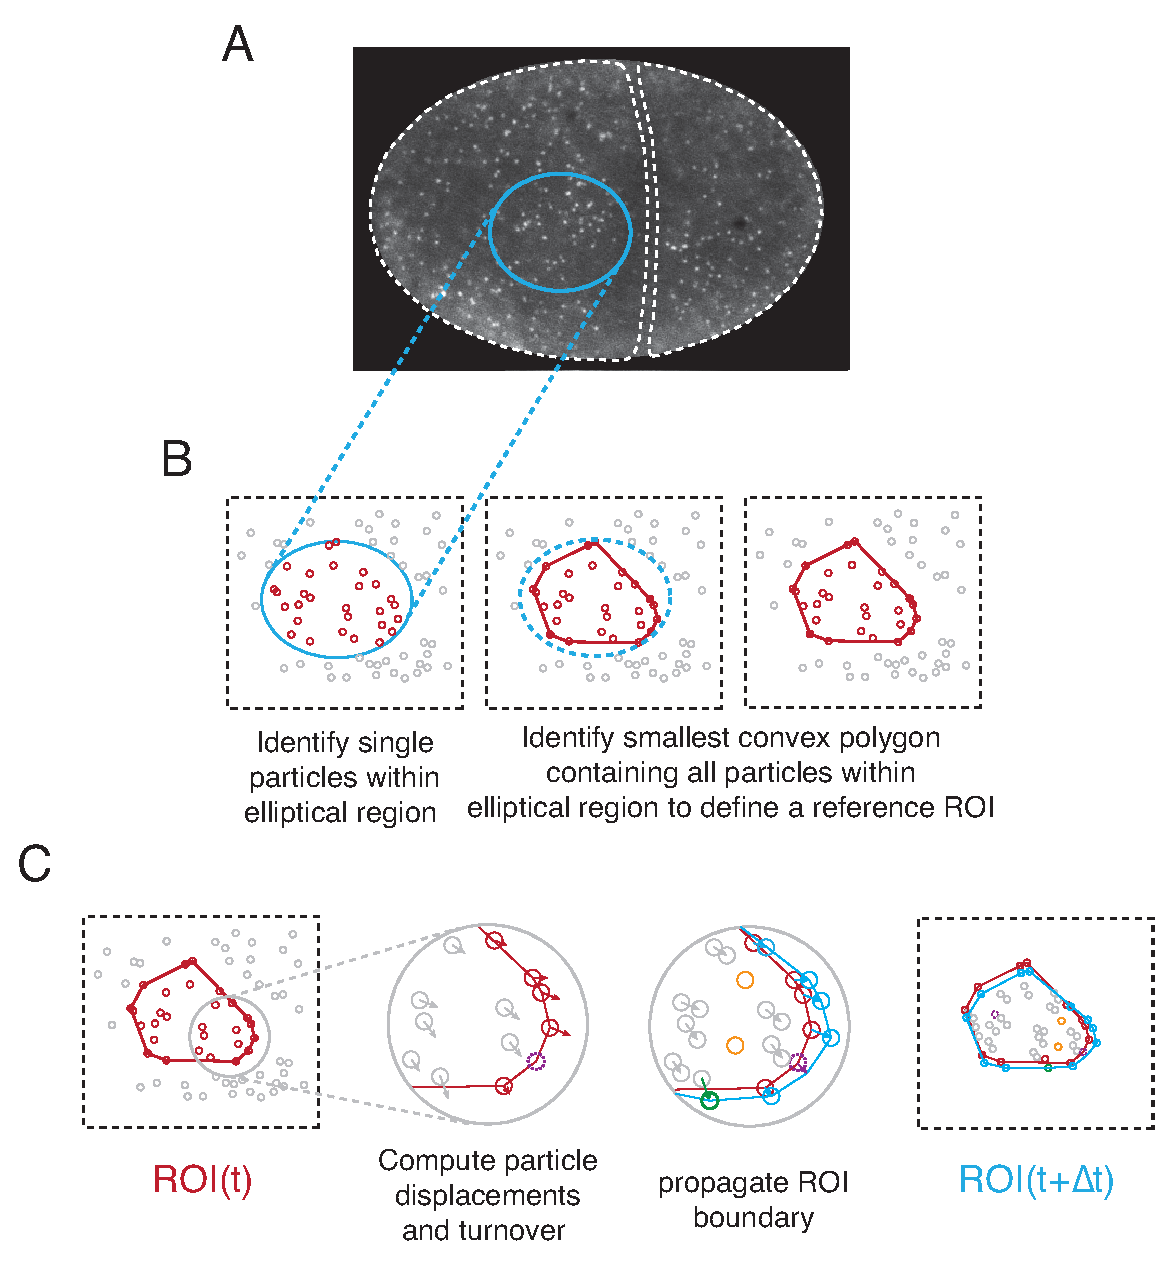
\includegraphics[width=0.7\textwidth]{pulse/Figure2-10}

\caption[Schematic overview of methods for tracking a moving and deforming patch of cortex from single molecule data.]{\label{fig:2210} \textbf{Schematic overview of methods for tracking a moving and deforming patch of cortex from single molecule data.} (A) Micrograph of a two-cell stage embryo expressing Actin::GFP at single-molecule levels. Anterior is to the left.  Dashed lines indicate the outlines of AB and P1.  The blue ellipse identifies a region in which a pulse occurs, from which a ``reference ROI'' will be extracted. (B) Method for extracting the reference ROI. Left:  Single particles detected in the raw image.  The particles shown in red are those contained within the blue ellipse.  Middle and right: The reference ROI (solid red line) is the smallest convex polygon containing all red particles. (C) Strategy for iterative propagation of the polygonal ROI from frame to frame (either backwards or forwards in time).  The polygon’s vertices move with the particle that defined that vertex so long as the particle remains visible. When a particle associated with a vertex disappears (dashed magenta particle in middle left panel), the vertex displacement is extrapolated from the motion of the surrounding particles. If an internal particle moves outside the boundaries of the polygon defined by existing vertices (green particle in middle right panel) a new vertex associated with that particle is introduced.}
\end{figure}




%Figure \ref{fig:221}1

\begin{figure}[!htbp]
\centering
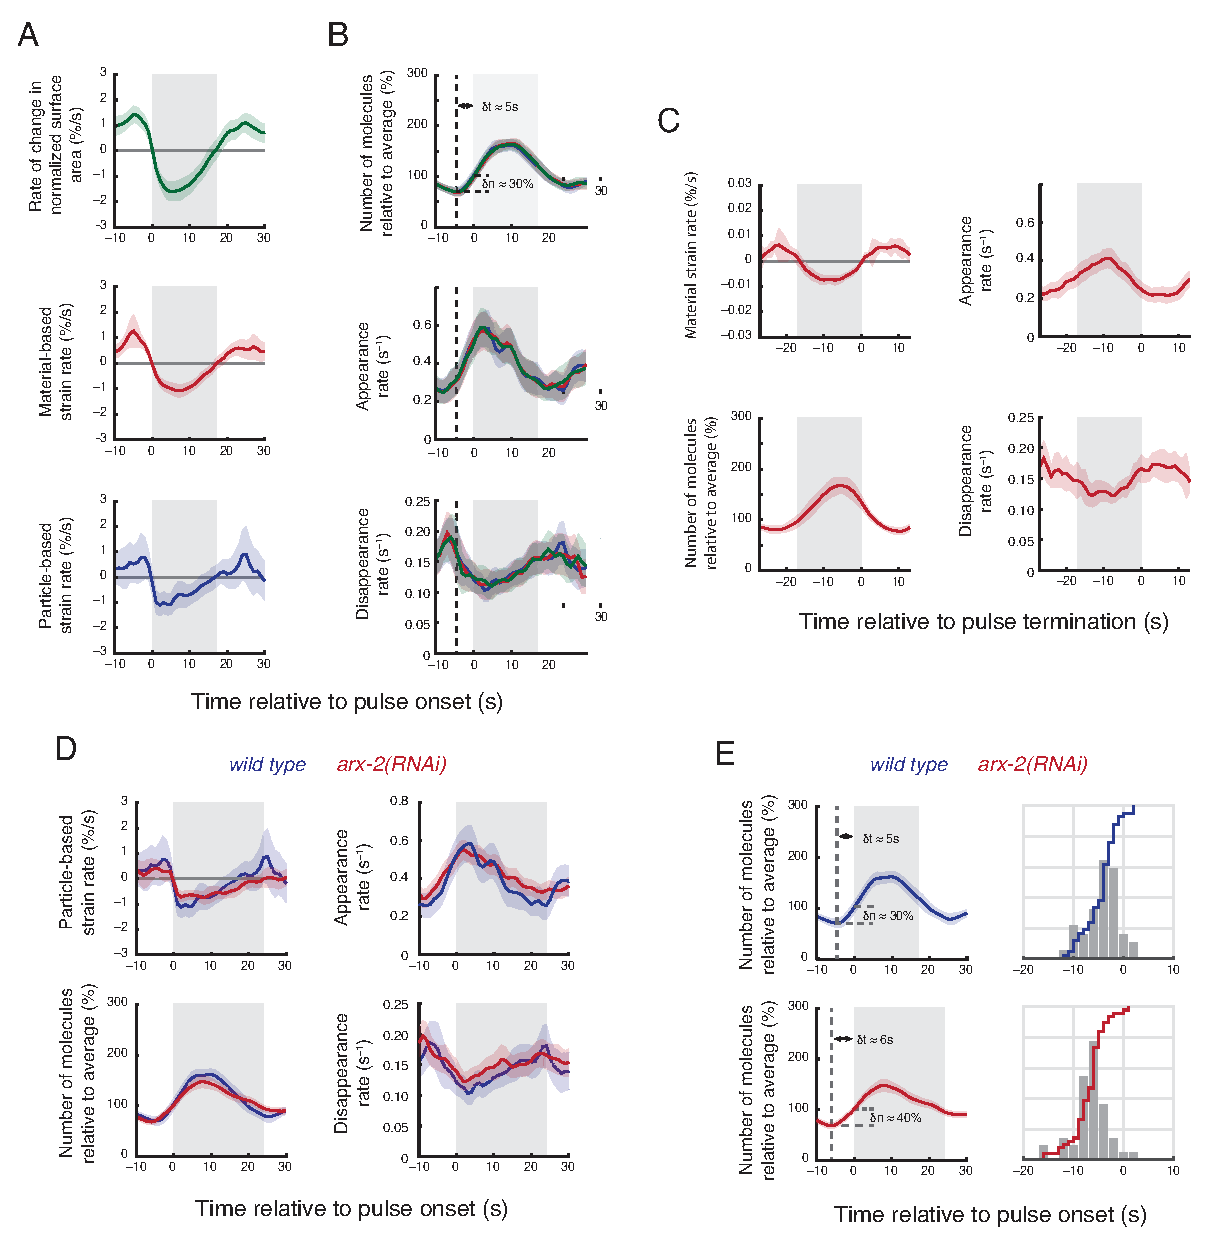
\includegraphics[width=0.4\textwidth]{pulse/Figure2-11}

\caption[Comparison of different methods to quantify local deformation (strain rate) and to align data across multiple pulses.]{ \label{fig:2211} \textbf{Comparison of different methods to quantify local deformation (strain rate) and to align data across multiple pulses.} (A,B) Comparison of different methods used to compute local deformation rates during pulses. (A) Measures of deformation rate vs time for the same data using three different metrics: (top) Rate of change in normalized surface area, (middle) material strain rate and (bottom) particle based strain rate (see materials and methods for details on how these were computed). (B) Measurements of single molecule number (top), appearance rate (middle) and disappearance rate (bottom) were aligned and averaged with respect to the onset of contraction, over 42 pulses, using the three metrics to measure deformation: change in normalized surface area (green), material strain rate (red), and particle-based strain rate (blue). Vertical dashed lines mark lowest actin density preceding the pulse. Horizontal dashed lines in top graph mark, respectively, the minimum number of actin molecules and the number of molecules at the onset of contraction. For all three metrics, the delay from actin minimum to contraction onset is $\delta$t $\approx$ 5s, and the relative change in number of molecules from minimum to contraction onset is $\delta$n $\approx$ 30$\%$. (C) Measurements of material strain rate, number of molecules, appearance rate and disappearance rate, aligned and averaged with respect to the end of contraction for the same data shown in A\&B. (D) Measurements of particle-based strain rate, number of molecules, appearance rate and disappearance rate, aligned and averaged with respect to the onset of contraction, in wild type (blue, n = 42 pulses) and \textit{arx-2}(RNAi) (red, n = 49 pulses) embryos. (E) Left column: number of molecules relative to average in wild type (blue) and \textit{arx-2}(RNAi) (red) embryos, as previously displayed in (D). The vertical dashed line marks lowest actin density preceding the pulse, delayed respectively by $\delta$t $\approx$ 5s and $\delta$t $\approx$ 6s from the contraction onset (gray box). The horizontal dashed line displays the amount of pre-contraction increase in the number of actin molecules, with $\delta$n $\approx$ 30$\%$ and $\delta$n $\approx$ 40$\%$, respectively. Right column: a histogram showing the distribution of delays between contraction onset and increase of actin molecules. Staircase line: cumulative distribution function of the delays. Error bars report 95$\%$ confidence intervals.}
\end{figure}







%Figure \ref{fig:221}2
\begin{figure}[!htbp]
\centering
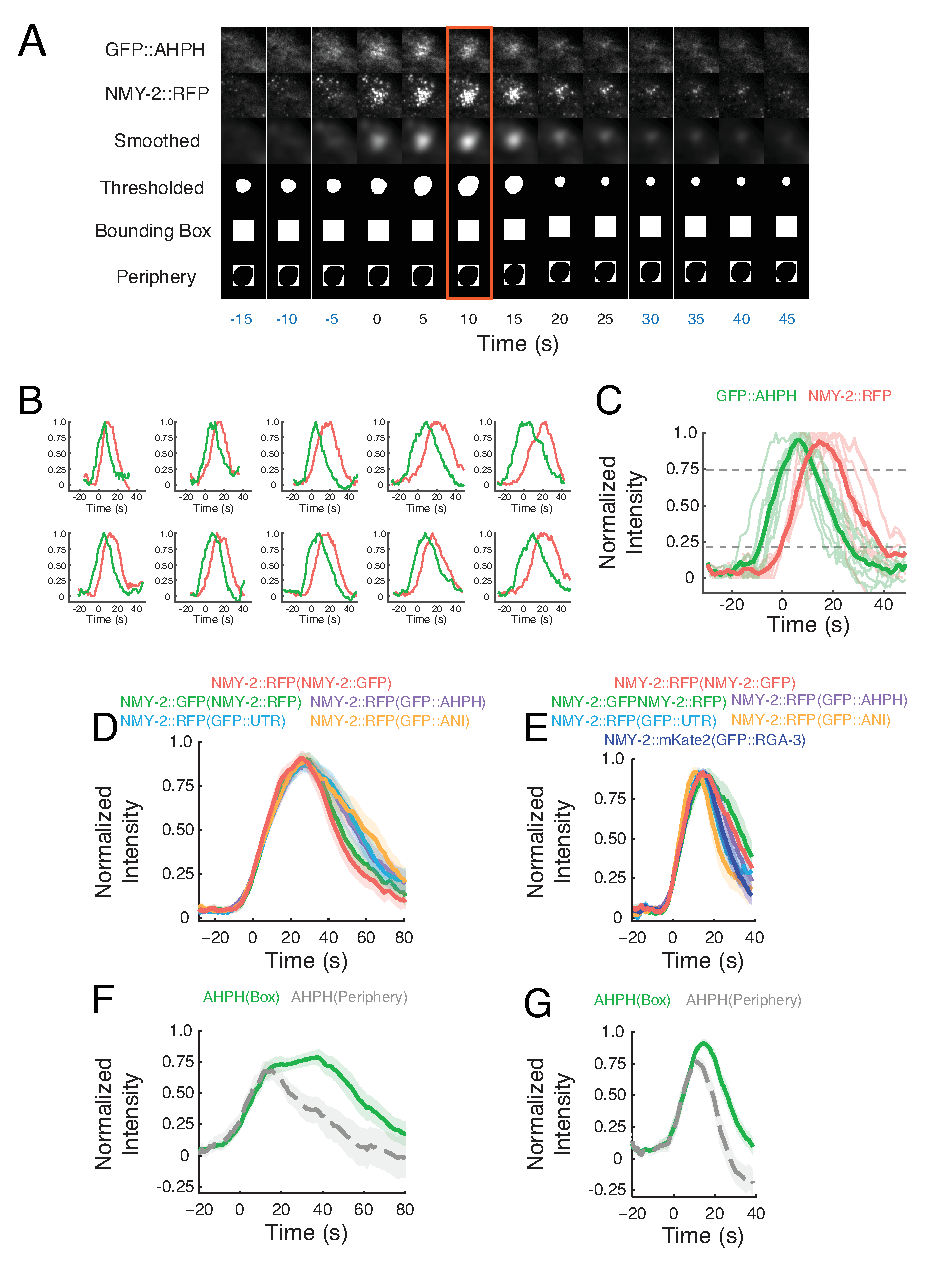
\includegraphics[width=0.5\textwidth]{pulse/Figure2-12}

\caption[Schematic overview of methodology for measuring and aligning fluorescence intensities from two-color data during pulsed contractions.]{ \label{fig:2212} \textbf{Schematic overview of methodology for measuring and aligning fluorescence intensities from two-color data during pulsed contractions.} (A) Method for determining regions of interest in which to measure fluorescence intensities, illustrated for a single pulse.  Row 1:  raw GFP::AHPH signal. Row 2: raw NMY-2::RFP signal.  Row 3: smoothed NMY-2::RFP signal. Row 4: thresholded NMY-2::RFP signal. Row 5: The smallest box containing the largest thresholded domain is the bounding box.  In each frame, the center of bounding box is located on the centroid of the thresholded domain. Row 6: A fixed-size peripheral region is the complement of the largest thresholded region within its bounding box.      The center of the fixed-size peripheral region is located at the center of the thresholded region in each frame.  (B) Normalized fluorescence intensity of GFP::AHPH and NMY-2::RFP versus time for ten representative pulses in AB cells. Time t = 0 when NMY-2::RFP rises above 25$\%$ of its normalized maximum value. (C) Fluorescence intensities from all pulses in (B) co-aligned relative to time t = 0. The bold traces represent the average GFP::AHPH and NMY-2::RFP intensities. (D,E) Alignment of averaged normalized fluorescence intensities for NMY-2::XFP measured for pulses in P0 (D) and AB (E) cells co-expressing the indicated probes (shown in parentheses). Time t = 0 is when NMY-2::XFP rises above 25$\%$ of its normalized maximum value. (F,G) Averaged normalized fluorescence intensity of GFP::AHPH measured in the bounding box (green) and periphery (gray) for pulses in P0 (F) and AB (G) cells.  In (D-G), halos report 95$\%$ confidence intervals.}
\end{figure}
















%Figure \ref{fig:221}3
\begin{figure}[!htbp]
\centering
\includegraphics[width=0.6\textwidth]{pulse/Figure2-13}

\caption[Two color analysis of Myosin II and Anillin dynamics during pulsed contractions in one- and two-cell embryos.]{ \label{fig:2213} \textbf{Two color analysis of Myosin II and Anillin dynamics during pulsed contractions in one- and two-cell embryos.}(A,E) Micrographs of two-cell (A) and one-cell (E) embryos co-expressing GFP::ANI-1 and NMY-2::RFP. White arrowheads indicate individual pulses. (B,F) Expanded views of single pulses illustrating temporal dynamics of GFP::ANI-1 and NMY-2::RFP accumulation. (C,G) Plots of averaged normalized fluorescence intensities for NMY-2::RFP and GFP::ANI-1 from two-color movies, aligned to the time at which NMY-2::RFP reaches 25$\%$ threshold. The averaged normalized fluorescence intensity of GFP::AHPH, co-aligned using the NMY-2::RFP signal, is shown for reference. Halos report 95$\%$ confidence intervals. (D,H) Distribution of the delays in the onset of appearance and disappearance of GFP::ANI-1 measured relative to NMY-2::RFP.  Onset of appearance and disappearance were measured respectively as the time at which the normalized signal rose above 25$\%$ or fell below 75$\%$ of the maximum value. }
\end{figure}




%Figure \ref{fig:221}4
\begin{figure}[!htbp]
\centering
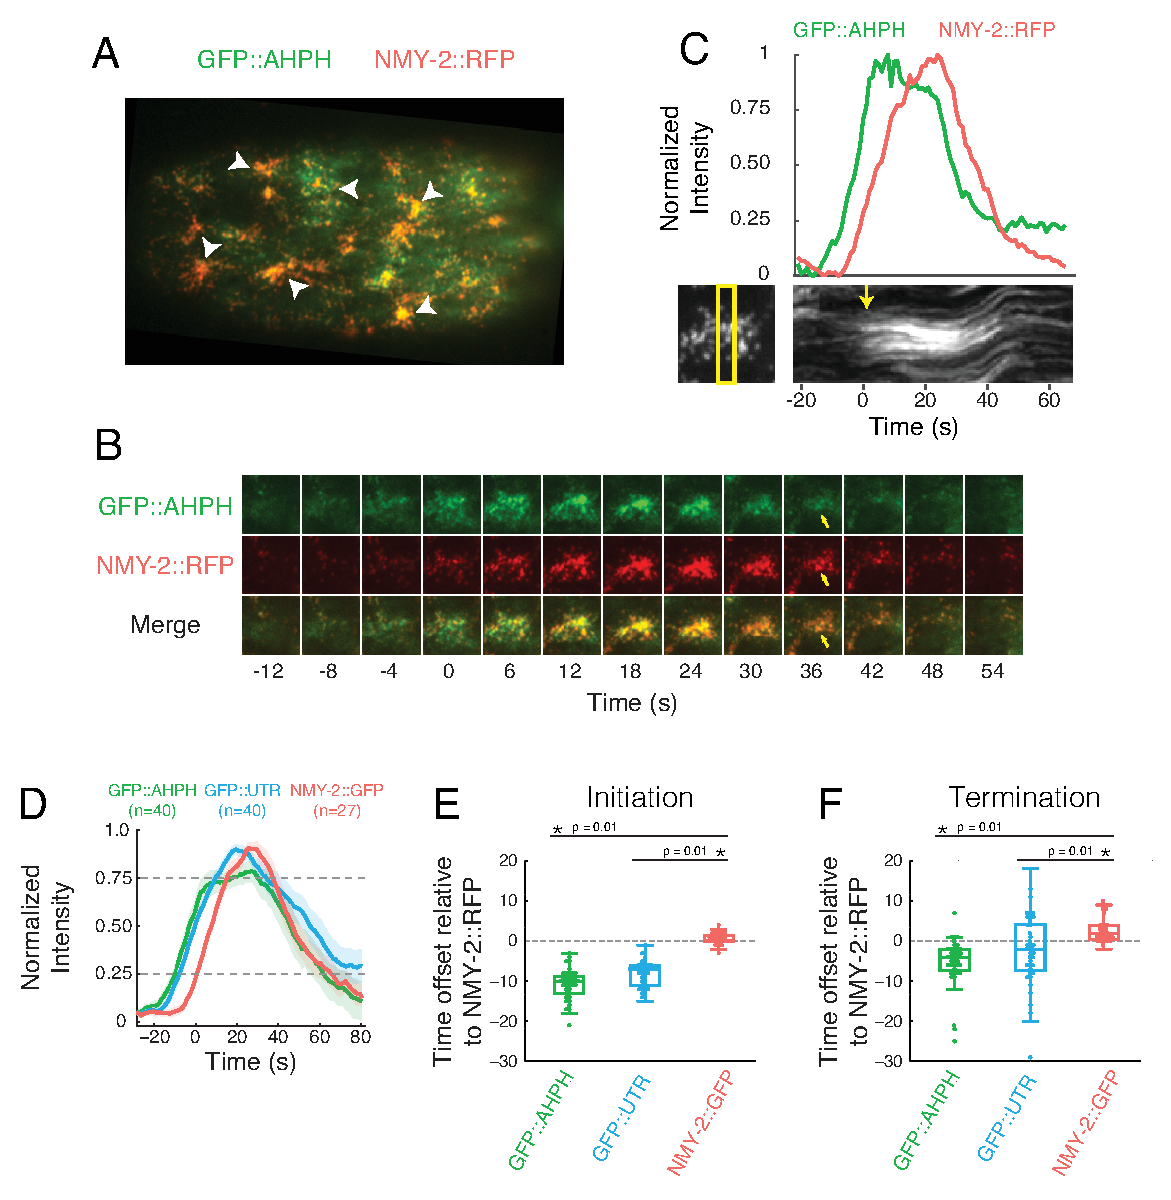
\includegraphics[width=0.65\textwidth]{pulse/Figure2-14}

\caption[Two color analysis of pulsed contractions in P0.]{\label{fig:2214} \textbf{Two color analysis of pulsed contractions in P0.} (A) A zygote expressing GFP::AHPH and NMY-2::RFP. White arrowheads indicate individual pulses. (B) Expanded view of a single pulse illustrating temporal dynamics of GFP::AHPH and NMY-2::RFP accumulation. Time delay between frames is 4s for the first 4 frames, and 6s thereafter. (C) Plot of normalized fluorescence intensities of GFP::AHPH and NMY-2::RFP versus time for the pulse displayed in (B). Below: kymograph showing movements of NMY-2::RFP punctae before and during the pulse. Yellow box at left indicates the region used to make kymograph. Yellow arrow at right indicates the onset of contraction. Note that a sharp rise in GFP::AHPH precedes both Myosin accumulation and onset of contraction. (D) Averaged normalized fluorescence intensities for NMY-2::RFP, GFP::AHPH and GFP::UTR from two-color movies, aligned to the time at which NMY-2::RFP reaches 25$\%$ threshold. Halos report 95$\%$ confidence intervals. (E) Distributions of the delay in onset of accumulation of GFP::AHPH, GFP::UTR, and NMY-2::GFP, measured relative to the onset of accumulation of NMY-2::RFP during pulse initiation for many individual pulses. Onset of accumulation is measured as the time at which each normalized signal exceeds 25$\%$ of its maximum value. (F) Distributions of the delay in the onset of disappearance of GFP::AHPH, GFP::UTR, and NMY-2::GFP measured relative to NMY-2::RFP during pulse termination for many individual pulses. Onset of disappearance is measured as the time at which each normalized signal falls below 75$\%$ of its maximum value. In (E,F) box plots, the central mark represents the median, the box indicates the 25th and 75th percentile, the whiskers mark the minimum and maximum values and the ``+'' symbol represents outliers.}
\end{figure}






